\documentclass[dissertation]{dissertation-gwu}[2019/11/25]
% \documentclass[thesis]{thesis-gwu}[2018/08/31]

\usepackage[boxed]{algorithm}
\usepackage{algorithmic}
\usepackage{amssymb}
\usepackage{array}
\usepackage{booktabs}
\usepackage{caption}
\usepackage{csquotes}
\usepackage{float}
\usepackage{graphicx}
\usepackage{listings}
\usepackage{makecell}
\usepackage{pdfpages}
\usepackage{setspace}
\usepackage{subfiles}
\usepackage[dvipsnames]{xcolor}

\algsetup{linenosize=\small}

\captionsetup[boxed]{skip=16pt}
\captionsetup[table]{skip=0.9pt}

\DeclareMathAlphabet{\mathcal}{OMS}{cmsy}{m}{n}

\let\Algorithm\algorithm
\renewcommand\algorithm[1][]{\Algorithm[#1]\setstretch{1.2}}

\let\oldemptyset\emptyset
\let\emptyset\varnothing

\lstset{
  language=R,
  basicstyle=\color{black}\linespread{0.95}\scriptsize\ttfamily,
  commentstyle=\color{gray},
  keywordstyle=\color{black},
  stringstyle=\color{blue},
  abovecaptionskip=16pt,
  captionpos=b,
  frame=single,
  rulecolor=\color{black},
  numbers=left,
  numberstyle=\scriptsize\ttfamily\color{gray},
  stepnumber=1,
  numbersep=5pt,
  breaklines=true,
  breakindent=5pt,
  breakatwhitespace=true,
  postbreak=\mbox{\textcolor{red}{$\hookrightarrow$}\space},
  showstringspaces=false,
  showtabs=false,
  tabsize=2}

% \begin{filecontents}{tex/doe-o-474.tex}
% \cleardoublepage\phantomsection
% \addcontentsline {toc}{chapter}{DOE Order 474.2, Table C. Graded Safeguards Table}
% \centering
% \includepdf[pages=1,pagecommand=\label{ch:doe-o-474},angle=90,trim=0.5cm 1.5cm 0 0]{figures/doe-o-474.pdf}
% \end{filecontents}

\newcommand{\ind}{\perp \!\!\! \perp}

% !TEX root = ../dissertation.tex

% title
\title{Analysis of Process Criticality Accident Risk Using a \texorpdfstring{\\}{} Metamodel-Driven Bayesian Network}

% author
\author{William John Zywiec}

% previous degrees
\bsdepartment{Nuclear Engineering}
\bsschool{Rensselaer Polytechnic Institute}
\bsgrad{May 2013}

\msdepartment{Systems Engineering}
\msschool{The Johns Hopkins University}
\msgrad{May 2017}
\showmsdegree
% \hidemsdegree

% PhD degree commands
% committee
\showcommitteepage
% \hidecommitteepage 
\committee{
  Shahram Sarkani, Professor, Dissertation Director\\\\
  Thomas Andrew Mazzuchi, Professor, Dissertation Co-Director}

% chair must be entered separately for formatting reasons
\chair{Shahram Sarkani}
\chairtitle{Professor}
\cochair{Thomas Andrew Mazzuchi}
\cochairtitle{Professor}
\department{Engineering Management and Systems Engineering}

\phdgrad{November X, 2020}
\defensedate{November X, 2020}
% year of completion for copyright page
\year=2020

% copyright page
% \copyrightholder{someone else}

% dedication
\dedication{
  \begin{center}
    For my family.
  \end{center}}

% acknowledgments
\acknowledgments{
  I would like to thank my wife, Katrina, for supporting me throughout my undergraduate and graduate education, and for going along with my decision to pursue a PhD.
  I would also like to thank my advisors, Dr. Shahram Sarkani and Dr. Thomas Mazzuchi, for providing invaluable advice and guidance, and for putting together and managing an excellent program.
  Additional thanks go to Daniel Falbel, for answering questions about \textit{TensorFlow}, and Dr. Shankar Kulumani, for putting together the \LaTeX\ template I used to write this dissertation.
  Lastly, I would like to thank David Heinrichs and Dr. Thomas McLaughlin, because "if I have seen further it is by standing on the shoulders of giants."}

% choose preface, prologue, or foreword

% preface
\preface{}

% prologue
\prologue{}

% foreword
\foreword[2]{}

% show/hide front matter pages
\showcopyright
\showabstract
\showcommitteepage
\showdedication
\showacknowledgments
\hidepreface
\hideprologue
\hideforeword

% table of contents
% show/hide lists of figures, tables, etc.
\showlistoffigures
\showlistoftables
\hidenomenclature 
\hidelistofabbreviations
\hidelistofsymbols

% the glossaries package automatically turns off lists of abbreviations and symbols
\setabbreviationstyle[acronym]{long-short}
\setabbreviationstyle[abbreviation]{long-short}
\makeglossaries

% show/hide the glossaries page
\showglossarieslistofabbreviations
\hideglossarieslistofsymbols
\hideglossariesglossaryofterms

\loadglsentries{tex/glossaries-abbreviations.tex}
% \loadglsentries{tex/glossaries-symbols.tex}
% \loadglsentries{tex/glossaries-terms.tex}

% abstract
\abstract{
  Since the discovery of fission in 1938, there have been more than 60 criticality accidents throughout the world.
  These accidents are divided into two categories: those that occur during critical experiments or operations with research reactors, and those that occur in production facilities, more commonly referred to as \textit{process criticality accidents}.
  The focus of this work is on the development of a methodology that uses a Bayesian network and a neural network metamodel to estimate process criticality accident risk.}


\begin{document}

  % !TEX root = ../dissertation.tex
% !TEX root = ../introduction.tex

\chapter{Introduction}

A criticality accident is an uncontrolled fission chain reaction that occurs when fissionable material (e.g., plutonium, uranium) is inadvertently assembled into a critical or supercritical mass.
Since the discovery of fission in 1938 \cite{hahn}, there have been more than 60 criticality accidents throughout the world \cite{mclaughlin}.
These accidents are divided into two categories: those that occur during critical experiments or operations with research reactors, and those that occur in production facilities, more commonly referred to as \textit{process criticality accidents} \cite{mclaughlin}.
The focus of this work is on the development of a methodology that uses a Bayesian network and a neural network metamodel to estimate process criticality accident risk.

For those who are unfamiliar with criticality accidents, there is the \gls{ines}, which was introduced in 1990 by the \gls{iaea}, to enable prompt communication of the safety significance of accidents and incidents to a wider audience \cite{ines}.
\gls{ines} goes from 0 to 7 and is intended to be logarithmic, with each level representing an accident approximately ten times as severe as the next level down.
The Chernobyl disaster, for example, was an \gls{ines} level 7 event, which is defined as a "major release of radioactive material with widespread health and environmental effects requiring implementation of planned and extended countermeasures" \cite{ines}.
On the other end of the scale is an \gls{ines} level 0 event, which is a "deviation" with no off-site consequences \cite{ines}.
Process criticality accidents are typically reported as \gls{ines} level 3 or 4 events, which are defined as either a "serious incident" or an "accident with local consequences" \cite{ines,kermisch}.

Historically, fault tree analysis has been the main methodology used by the \gls{doe} to estimate process criticality accident risk \cite{doe2013}.
Fault tree analysis consists of defining one or more initiating events, building logic gates for all foreseeable failure paths, and applying Boolean algebra to calculate the top-level failure probability \cite{roberts}.
Over the years, several improvements have been made to this methodology by incorporating binary decision diagrams \cite{reay,remenyte}, dynamic fault trees \cite{cepin,ruijters}, and Monte Carlo simulations \cite{rao}.
However, fault tree analysis still relies heavily on identifying events, failure paths, and minimum cut sets, which is difficult to do for fissionable material operations and other systems with a high degree of dimensionality \cite{au,cadini2016,khakzad}.

For operations with fissionable material, there are ten parameters that affect nuclear criticality: mass, absorption, geometry/shape, interaction, concentration/density, moderation, enrichment, reflection, volume, and temperature \cite{knief}.
Most parameters are observable, but even with a perfect understanding of all ten, a radiation transport code is still needed to calculate the effective neutron multiplication factor ($k_{eff}$) of the system, in order to determine if a criticality accident will occur.
A simplified form of the equation to calculate $k_{eff}$ is shown in \ref{eq:keff} \cite{lamarsh}.
%
\begin{equation}
  \label{eq:keff}
  k_{eff} = \frac{\mbox{neutrons produced from fission in one generation}}{\mbox{neutrons produced from fission in the previous generation}}
\end{equation}

If $k_{eff} < 1$, the system is subcritical---and presumably safe.
If $k_{eff} \geq 1$, the system will produce either a self-sustaining or divergent fission chain reaction and an accompanying burst of neutron and gamma ray radiation (i.e., a criticality accident) \cite{knief,lamarsh}.
For nuclear criticality applications, $k_{eff}$ is typically calculated using a Monte Carlo radiation transport code, such as MCNP \cite{mcnp}.
A Monte Carlo radiation transport code works by reading input and building a computer model of the system, which consists of a specific geometric arrangement of fissionable and non-fissionable materials.
The code then simulates particle interactions and calculates a probabilistic value for $k_{eff}$, based on the number and types of interactions that occur (e.g., fission, scattering, absorption) \cite{mcnp}.

In this work, a Bayesian network is used to model parameters (or variables) that affect nuclear criticality, and a neural network metamodel is trained to predict $k_{eff}$, based on calculations that were performed using MCNP \cite{mcnp} and \gls{endf}/B-VII.1 nuclear data \cite{chadwick2011}.
This work also describes how this methodology is applied to fissionable material operations in the Plutonium Facility (Building 332) at Lawrence Livermore National Laboratory.
Building 332 is a multi-laboratory facility that supports a wide variety of activities that are sponsored by the \gls{nnsa} \cite{doe2005}.
Although the risk of a process criticality accident in Building 332 is low \cite{doe2005}, the consequences are extreme, due to the impact a criticality accident would have on the safety and stewardship of the United States' nuclear stockpile \cite{opus,dod}.

% -----------------
% Literature Review
% -----------------

\section{Literature Review}

The motivation for this work originated while reviewing Environmental Impact Statements for U.S. Department of Energy sites and noting that radiation transport codes were not used to analyze the frequency or severity of process criticality accidents (Table \ref{table:doe}).
At the time, this was considered somewhat strange, since radiation transport codes are commonly used in the field of nuclear engineering to design experiments and evaluate fissionable material operations in nuclear facilities.
After further review, it appeared that most \gls{doe} Environmental Impact Statements use a simplified form of fault tree analysis, which relies on overly broad and unrealistic assumptions of accident conditions \cite{mattson}.

\begin{table}
  \caption{Process criticality accident risk at U.S. Department of Energy sites}
  \label{table:doe}
  \renewcommand\arraystretch{1.5}
  \begin{center}
    \begin{tabular}{|l c c|}
      \hline
                                             & accidents/year & reference \\
      \hline
      Lawrence Livermore National Laboratory & 3.2e-05        & DOE/EIS-0348 \\
      Los Alamos National Laboratory         & $<$ 1e-04      & DOE/EIS-0283 \\
      Nevada National Security Site          & $\leq$ 1e-02   & DOE/EIS-0426 \\
      Pantex Plant                           & $<$ 1e-06      & DOE/EIS-0098 \\
      Sandia National Laboratories           & $<$ 1e-07      & DOE/EIS-0281 \\
      Savannah River Site                    & 1e-02          & DOE/EIS-0541 \\
      Y-12 National Security Complex         & $\leq$ 1e-02   & DOE/EIS-0387 \\
      \hline
    \end{tabular}
  \end{center}
\end{table}

A summary of the \gls{sar} at the Rocky Flats Plant \cite{mattson} provides some insight into how \gls{doe} sites estimate process criticality accident risk.
The following paragraphs are taken from R.J. Mattson \cite{mattson}:

\begin{displayquote}

  \textit{The \gls{sar} provides the frequencies for groups of initiating events but does not provide any information on the causes for individual initiating events within a group.
  A particular concern is the treatment of human errors.
  Although the involvement of humans in the process is mentioned, the treatment of human errors in the risk analysis is not addressed.
  The \gls{sar} does not include sufficient detail.
  At least basic assumptions and data, as well as the process, used to derive the results need to be documented.
  The example calculation in Appendix C of the \gls{sar} is insufficient.}

  \vspace{+0.4cm}

  \textit{Further, in the course of calculating the risk of criticality accidents, there has not been a systematic, detailed study of the specific operations performed at the Rocky Flats Plant, nor an estimate of the associated probability of human error.
  Such a study might well produce results different from those resulting from generic data for human error that were used.
  Of even more importance to safe operation at the plant is the fact that a detailed study of the plant-specific operations might identify possibilities for human error that have not yet been observed.
  This could be a rich source of new safety information.}

\end{displayquote}

\noindent Even though this summary was published in 1989, it is still relevant today.
The \gls{sar} that is referenced was written in 1987, and it estimated the site-wide risk of a criticality accident to be 3e-04 accidents/year---six years before a process criticality accident nearly occurred in Building 771 \cite{mckamy}.

% -----------------------
% -----------------------
% -----------------------

To illustrate the complexity of fissionable material operations, the results of two different sets of MCNP calculations are plotted and shown in Figures \ref{fig:contour1} and \ref{fig:contour2}.
The first plot represents a sphere of alpha-phase plutonium ($\rho = 19.86$ g/cm$^{3}$) homogeneously dispersed in water, with one inch of water reflection (Figure \ref{fig:contour1}).
The second plot represents a sphere of alpha-phase plutonium homogeneously dispersed in magnesium oxide, with one inch of water reflection (Figure \ref{fig:contour2}).
Even though the only difference between these plots is moderation, the $k_{eff}$ contours are much different (Figure \ref{fig:contour2})---and these differences compound when other parameters that affect nuclear criticality are changed \cite{knief}.

\begin{figure}
  \centering
  \includegraphics[width=\textwidth]{figures/contour1.png}
  \caption{\textit{keff} contour plot of a sphere of alpha-phase plutonium (95\% $^{239}$Pu, 5\% $^{240}$Pu by weight) with water moderation and one inch of water reflection}
  \label{fig:contour1}
  \vspace{+1.1cm}
  \includegraphics[width=\textwidth]{figures/contour2.png}
  \caption{\textit{keff} contour plot of a sphere of alpha-phase plutonium (95\% $^{239}$Pu, 5\% $^{240}$Pu by weight) with magnesium oxide moderation and one inch of water reflection}
  \label{fig:contour2}
\end{figure}

\subsection{Bayesian Network}

The modeling of high-dimensional, nonlinear systems led to the selection of a Bayesian network \cite{pearl} as one-half of the methodology described in this work.
One benefit of using a Bayesian network is that complex mechanisms leading to top-level failure do not need to be well understood prior to building the model \cite{khakzad,pearl,scutari}.
The only things that are needed are an understanding of parameters that affect nuclear criticality \cite{knief} and the ability to model each one.
Another benefit of using a Bayesian network is that a single network can model multiple modes and/or causes of failure \cite{bobbio,tien}.
Both of these benefits are ideal for this application, since it is generally easier to model parameters and estimate probabilities when there isn't a need to evaluate low- or mid-level failure.
One downside of using a Bayesian network is that its ability to model latent variables (e.g., $k_{eff}$) is constrained by the size and complexity of the model \cite{koller,tien}.
Existing methods, such as \gls{form} or \gls{sorm}, use a Taylor series expansion to approximate the “most probable failure point”, while others use Monte Carlo variance reduction techniques to select samples that are in the "vicinity of failure" \cite{cadini2016}.
Recently, a new class of methods have been developed, which use a sampling algorithm coupled to a surrogate model (or \textit{metamodel}) to approximate a performance function \cite{cadini2016}.

\subsection{Neural Network Metamodel}

The neural network metamodel described in this work is based on prior research in the field of structural engineering, which focuses on using metamodels to reduce the computational burden of performing direct, simulation-based analysis of physical systems \cite{cadini2015,dubourg,papadrakakis,raissi,zhang}.
There are several different types of metamodels that can be used to approximate a performance function, including Gaussian process regression models \cite{dubourg,quinonero,smola}, neural networks \cite{goodfellow,hinton}, polynomial chaos expansions \cite{blatman,crestaux,oladyshkin}, quadratic response surfaces \cite{ames,hartley}, random forests \cite{kuhn,liaw}, and support vector machines \cite{bennett,scholkopf,suykens}.
Neural networks were selected for further use in this work, based on two white papers \cite{tensorflow} that describe \gls{gpu}-accelerated tensor operations (i.e., vector and matrix calculations), which neural networks are preconfigured to use \cite{tensorflow,keras}.
After initially renting \gls{gpu}-hours on the Amazon Elastic Compute Cloud (EC2), I built a computer with an NVIDIA GeForce GTX 1080 8 GB GDDR5X \gls{gpu}, specifically to work on this dissertation.

\subsection{Random Sampling Algorithms}

The methodology described in this work is based on random sampling algorithms described in F. Cadini and A. Gioletta \cite{cadini2016}, F. Cadini et al. \cite{cadini2015}, V. Dubourg et al. \cite{dubourg}, D. Koller and N. Friedman \cite{koller}, and M. Papadrakakis and N.D. Lagaros \cite{papadrakakis}.

\subsection{Software Packages}

The \textit{bnlearn} \cite{bnlearn}, \textit{Keras} \cite{keras}, and \textit{TensorFlow} \cite{tensorflow} software packages were used throughout this work.
These software packages were selected because they are popular, well documented, and written in R, a programming language that has several graphical and statistical software packages that were also used throughout this work \cite{igraph,fitdistrplus,grain,caret,bnlearn,ggplot2}.
\textit{bnlearn} \cite{bnlearn} was used to build the Bayesian network and generate random samples.
Other Bayesian network software packages, including BUGS and JAGS, were also considered, but not selected, due to lack of integration with either Python or R.
The \textit{Keras} \cite{keras} and \textit{TensorFlow} \cite{tensorflow} software packages were used to build the neural network metamodel.
\textit{Keras} is a high-level \gls{api}, which manages interactions between Python/R and the \textit{TensorFlow} platform \cite{keras}.
\textit{TensorFlow} is an end-to-end, open source machine learning platform, which combines four key abilities \cite{tensorflow}:

\begin{itemize}
  \item Efficiently executing low-level tensor operations on \gls{cpu}s, \gls{gpu}s, and \gls{tpu}s
  \item Computing the gradient of arbitrary differentiable expressions
  \item Scaling computation to many devices
  \item Exporting programs to external servers, browsers, mobile, and embedded devices
\end{itemize}

\noindent \textit{Caffe} and \textit{PyTorch} were also considered, but not selected, due to being relatively new and untested when research for this work began in 2017.

% -------------
% Contributions
% -------------

\section{Contributions}

The primary contribution of this work is the development of a methodology that uses a Bayesian network and neural network metamodel to estimate process criticality accident risk.
Although neural network metamodels are not new, this work demonstrates the novel use of a metamodel in the context of performing a Bayesian network-based probabilistic risk assessment.
The main benefit of this methodology is that it combines the interpretability and random sampling algorithm of a Bayesian network with the high-dimensional, latent variable modeling capability of a neural network metamodel.
The secondary contribution of this work is the implementation and testing of a \gls{sse} loss function, which is shown to outperform the more commonly used \gls{mse} loss function.

\subsection{Publications}

  % !TEX root = ../dissertation.tex
% !TEX root = ../tex/mathematical-background.tex

% -----------------------
% Mathematical Background
% -----------------------

\chapter{Mathematical Background}

This chapter provides a mathematical background in nuclear criticality, Monte Carlo radiation transport, Bayesian networks, and neural networks.
The equations and figures included in this chapter, while not exhaustive, provide context for later sections of this work, which focus on building a coupled Bayesian network and neural network metamodel and using it to estimate process criticality accident risk.

% -------------------
% Nuclear Criticality
% -------------------

\section{Nuclear Criticality}

\textit{Nuclear fission} is an event that occurs when a target nucleus absorbs a neutron, transitions to an excited state, and then de-excites by splitting into two or more fission products and emitting neutron and gamma ray radiation (Figure \ref{fig:fission}).
This phenomenon was discovered on December 17, 1938 by Otto Hahn and Fritz Strassmann \cite{hahn}, and later explained on Feburary 11, 1939, in an article written by Lise Meitner and Otto Frisch \cite{meitner}.

\begin{figure}
  \centering
  \includegraphics[trim={1.5cm 5.6cm 1.5cm 3.9cm}]{figures/fission.pdf}
  \caption{Fission diagram}
  \label{fig:fission}
\end{figure}

% \begin{figure}
%   \centering
%   \includegraphics[width=\textwidth]{figures/yield.png}
%   \caption{$^{239}$Pu fission product yield \cite{chadwick2010}}
%   \label{fig:yield}
% \end{figure}

\textit{Nuclear criticality} is a self-sustaining or divergent fission chain reaction that occurs when fissionable material is assembled into a critical or supercritical mass \cite{knief}. 
Nuclear criticality is often expressed as a steady-state calculation of the \textit{effective neutron multiplication factor} ($k_{eff}$), which is the number of neutrons produced from fission in one generation, divided by the number of neutrons produced from fission in the previous generation (\ref{eq:keff}).
If the number of neutrons produced from fission in one generation is equal to the number of neutrons produced from fission in the previous generation, then the system is self-sustaining or critical ($k_{eff} = 1$).
If it is greater, the system is supercritical ($k_{eff} \geq 1$).
If it is less, the system is subcritical ($k_{eff} < 1$).

% ----------------------
% Nuclear Cross Sections
% ----------------------

\subsection{Nuclear Cross Sections}

Nuclear cross sections are used to describe the probability that a reaction will occur between a particle (e.g., a neutron) and a target nucleus (Figure \ref{fig:xs}).
The concept of a cross section is quantified in terms of "characteristic area", where a larger area means a larger probability of interaction.
The standard unit for measuring a nuclear cross section ($\sigma$) is the \textit{barn}, which is equal to 10$^{-24}$ cm$^{2}$ \cite{lamarsh}.

Nuclear cross sections depend on the size of the target nucleus, the type of reaction that occurs (e.g., fission, scattering, absorption, etc.), the energy of the incident particle, and, to a lesser extent, the temperature of the target nucleus and the relative angle between the incident particle and target nucleus.
Nuclear cross sections are also sometimes referred to as the \textit{microscopic cross sections}, to distinguish them from \textit{macroscopic cross sections}, which are weighted by the number density ($N$) of the target material (\ref{eq:xs}).
%
\begin{equation}
  \label{eq:xs}
  \Sigma_{t}(E) = N\sigma_{t}(E) = \mbox{macroscopic total cross section (cm$^{-1}$)}
\end{equation}

\noindent where \\
\indent $N = $ the number density of the target material (atoms/cm$^{3}$) \\
\indent $\sigma_{t} = $ the microscopic total cross section (cm$^{2}$) \\

The macroscopic total cross section represents the sum of all macroscopic cross sections for the target material, which includes capture ($\Sigma_{c}$), fission ($\Sigma_{f}$), scattering ($\Sigma_{s}$), and other rare events, such as ($n, \gamma$), ($n, p$), ($n, 2n$), and ($n, 3n$) reactions.
If a neutron is captured, it is considered to be removed from the system.
If a neutron, traveling in direction $\Omega$ at energy $E$, scatters off a target nucleus, it emerges from the scattering event with a new direction $\Omega^{\prime}$ and energy $E^{\prime}$.
The distribution of post-collision directions $\Omega^{\prime}$ and energies $E^{\prime}$ is expressed as $p(\Omega \cdot \Omega', E \rightarrow E')d\Omega'dE'$.

In Monte Carlo radiation transport codes, particle interactions are simulated by sampling the incremental probability of interaction per incremental distance traveled, as well as the angular and energy distributions, depending on the type of interaction that occurs.
Plots of these angular and energy distributions are shown in Figure \ref{fig:angle} and Figure \ref{fig:energy} for several different incident neutron energies.

\begin{figure}
  \centering
  \includegraphics[width=\textwidth]{figures/xs.png}
  \caption{$^{239}$Pu cross sections}
  \label{fig:xs}
\end{figure}

\begin{figure}
  \centering
  \includegraphics[width=\textwidth]{figures/angle.png}
  \caption{$^{239}$Pu elastic scattering angular distributions}
  \label{fig:angle}
\end{figure}

\begin{figure}
  \centering
  \includegraphics[width=\textwidth]{figures/energy.png}
  \caption{$^{239}$Pu (n,f) energy distributions}
  \label{fig:energy}
\end{figure}

% -------------------------------
% Monte Carlo Radiation Transport
% -------------------------------

\subsection{Monte Carlo Radiation Transport}

MCNP is a general-purpose Monte Carlo radiation transport code that is used throughout this work.
MCNP operates by reading input and building a computer model of the system, which consists of a specific geometric arrangement of fissionable and non-fissionable materials.
The code then simulates neutron interactions and calculates a probabilistic value for $k_{eff}$, based on the number and types of interactions that occur (e.g., fission, scattering, absorption) \cite{mcnp}.
The MCNP input deck, shown in Figure \ref{fig:input}, represents 500 grams of alpha-phase plutonium ($\rho =  19.86$ g/cm$^{3}$), homogeneously dispersed in a sphere of water, with one inch of water reflection (Figure \ref{fig:mcnp}).
The material cards are formatted by ZAID, which consists of a two-digit atomic number, a two- to three-digit mass number, and an alphanumeric suffix, which corresponds to an $xsdir$ data table entry and nuclear data files that are installed in the same directory as MCNP.
The ".80c" and ".20t" suffixes correspond to nuclear cross sections and S($\alpha,\beta$) thermal scattering treatments based on \gls{endf}/B-VII.1 \cite{chadwick2011}.

\begin{figure}
  \centering
  \lstinputlisting{source/500-alpha-h2o-13.97-none-sph.i}
  \caption{MCNP input deck}
  \label{fig:input}
\end{figure}

\begin{figure}
  \centering
  \includegraphics[scale=0.3]{figures/mcnp.png}
  \caption{MCNP model of 500 grams of alpha-phase plutonium homogeneously dispersed in a sphere of water, with one inch of water reflection}
  \label{fig:mcnp}
\end{figure}

There are seven source points specified in the MCNP input decks (Figure \ref{fig:input}): one at the origin, and six located along the positive and negative x, y, and z axes, at a distance from the origin equal to $2/3$ the radius of the sphere.
The \textit{kcode} data card is set to simulate random walks for 500 batches of 10,000 neutrons each (Figure \ref{fig:input}), from a randomly sampled Watt fission spectrum for $^{239}$Pu \cite{mcnp}.
After the first batch of random walks, the average number of neutrons produced from fission is tallied, and locations where fissions occur are selected as the new source points for the next batch.
The \textit{kcode} data card is set to only calculate $k_{eff}$ for batches 50 through 500, to ensure source points are evenly distributed throughout the system (Figure \ref{fig:input}).

There are three estimators that MCNP uses to calculate $k_{eff}$: collision, absorption, and track length.
The collision estimator is calculated using \ref{eq:keff-c}.
%
\begin{equation}
  \label{eq:keff-c}
  k_{eff}^{c} = \frac{1}{N} \sum_{i} W_{i} \frac{\sum_{k} f_{k} \bar{v}_{k} \sigma_{f_{k}}}{\sum_{k} f_{k} \sigma_{t_{k}}}
\end{equation}

\noindent where \\
\indent $k_{eff}^{c} = $ collision estimator \\
\indent $i$ is summed over all collisions in a cycle \\ 
\indent $k$ is summed over all isotopes of the target material involved in the $i^{th}$ collision \\
\indent $N = $ number of source particles \\
\indent $W_{i} = $ weight of collision particle \\
\indent $f_{k} = $ atom-fraction of isotope $k$ \\
\indent $\bar{v}_{k} = $ average number of neutrons produced from fission \\
\indent $\sigma_{f_{k}} = $ microscopic fission cross section \\
\indent $\sigma_{t_{k}} = $ microscopic total cross section \\

\noindent The fraction to the right of $W_{i}$ represents the number of neutrons produced from all fissions in the $i^{th}$ collision.
Multiplying this value by the weight of the collision particle ($W_{i}$), summing over all collisions in a cycle, and then dividing by the number of source particles results in the mean number of neutrons produced from fission for each cycle.
The absorption estimator is calculated using \ref{eq:keff-a}.
%
\begin{equation}
  \label{eq:keff-a}
  k_{eff}^{a} = \frac{1}{N} \sum_{i} W_{i} \bar{v}_{k} \frac{\sigma_{f_{k}}} {\sigma_{c_{k}} + \sigma_{f_{k}}}
\end{equation}

\noindent where \\
\indent $k_{eff}^{a} = $ absorption estimator \\
\indent $\sigma_{c_{k}} = $ microscopic capture cross section \\

\noindent The absorption estimator is only summed over the $i^{th}$ collision for the $k^{th}$ fissionable isotope.
This is different from the collision estimator, which is summed over all isotopes.
The track length estimator is calculated using \ref{eq:keff-t}.
%
\begin{equation}
  \label{eq:keff-t}
  k_{eff}^{t} = \frac{1}{N} \sum_{i} W_{i} \rho d \sum_{k} f_{k} \bar{v}_{k} \sigma_{f_{k}}
\end{equation}

\noindent where \\
\indent $k_{eff}^{t} = $ track length estimator \\
\indent $i$ is summed over all neutron trajectories \\
\indent $\rho = $ atomic density of the cell \\
\indent $d = $ neutron trajectory track length \\

\noindent MCNP takes the average of all $k_{eff}$ values for each estimator, for all active cycles, and uses it to calculate the \textit{maximum likelihood estimate} of $k_{eff}$ (\ref{eq:keff-mle}).
%
\begin{equation}
  \label{eq:keff-mle}
  k_{eff}^{x} = \frac{1}{C} \sum_{50}^{C} k_{eff,c}^{x}
\end{equation}

\noindent where \\
\indent $C = $ number of active cycles \\
\indent $k_{eff,\;c}^{x} = $ estimate of $k_{eff}$ for each active cycle \\

\noindent Assuming that the $k_{eff,\;c}^{x}$ for each estimator are independent, the sample standard deviation of the mean estimate of $k_{eff}$ can be obtained by \ref{eq:sd} \cite{urbatsch}.

\begin{equation}
  \label{eq:sd}
  \sigma_{\bar{k}_{eff}^{x}} = \frac{1}{\sqrt{C}} \sigma_{k_{eff}^{x}} = \left[ \frac{1}{C(C-1)} \sum_{c = 50}^{C} (k_{eff,\;c}^{x} - \bar{k}_{eff}^{x})^2 \right]^{1/2}
\end{equation}

\noindent where \\
\indent $\sigma_{\bar{k}_{eff}} = $ standard deviation of $\bar{k}_{eff}$ \\
\indent $\sigma_{k_{eff}} = $ standard deviation of each estimator's $k_{eff}$ values \\

\noindent The standard deviation of each estimator's $k_{eff}$ values are used to calculate the corresponding population covariance matrix (\ref{eq:cov}) \cite{urbatsch}.
%
\begin{equation}
  \label{eq:cov}
  \Sigma =
  \left[
  \begin{matrix}
    \sigma_{k_{eff}^{c}}^{2}  & \sigma_{k_{eff}^{ca}}^{2} & \sigma_{k_{eff}^{ct}}^{2} \\
    \sigma_{k_{eff}^{ac}}^{2} & \sigma_{k_{eff}^{a}}^{2}  & \sigma_{k_{eff}^{at}}^{2} \\
    \sigma_{k_{eff}^{tc}}^{2} & \sigma_{k_{eff}^{ta}}^{2} & \sigma_{k_{eff}^{t}}^{2}
  \end{matrix}
  \right]
\end{equation}

\noindent A square root solution of a $3 \times 3$ identity matrix is multiplied by $\Sigma$ (\ref{eq:cov}) and its transpose to obtain a $3 \times 3$ matrix, which further reduces to a $2 \times 2$ matrix with $i \times j$ ($\Sigma_{zij}$) submatrices (\ref{eq:cov-z}) \cite{urbatsch}.
%
\begin{equation}
  \label{eq:cov-z}
  \begin{split}
    \Sigma_{z} & = A \Sigma A^{T} \\
    & =
    \left[
    \begin{matrix}
      1 &  0 &  0 \\
      1 & -1 &  0 \\
      1 &  0 & -1
    \end{matrix}
    \right]
    \left[
    \begin{matrix}
      \sigma_{k_{eff}^{c}}^{2} & \sigma_{k_{eff}^{ca}}^{2} & \sigma_{k_{eff}^{ct}}^{2} \\
      \sigma_{k_{eff}^{ac}}^{2} & \sigma_{k_{eff}^{a}}^{2} & \sigma_{k_{eff}^{at}}^{2} \\
      \sigma_{k_{eff}^{tc}}^{2} & \sigma_{k_{eff}^{ta}}^{2} & \sigma_{k_{eff}^{t}}^{2}
    \end{matrix}
    \right]
    \left[
    \begin{matrix}
      1 &  1 &  1 \\
      0 & -1 &  0 \\
      0 &  0 & -1
    \end{matrix}
    \right] \\
    & =
    \left[
    \begin{array}{c|c c}
      \sigma_{c}^{2} & \sigma_{c}^{2} - \sigma_{ca}^{2} & \sigma_{c}^{2} - \sigma_{ct}^{2} \\
      \hline
      \sigma_{c}^{2} - \sigma_{ca}^{2} & \sigma_{c}^{2} + \sigma_{a}^{2} - 2\sigma_{ca}^{2} & \sigma_{c}^{2} + \sigma_{at}^{2} - \sigma_{ca}^{2} - \sigma_{ct}^{2} \\
      \sigma_{c}^{2} - \sigma_{ct}^{2} & \sigma_{c}^{2} + \sigma_{at}^{2} - \sigma_{ca}^{2} - \sigma_{ct}^{2} & \sigma_{c}^{2} + \sigma_{t}^{2} - 2\sigma_{ct}^{2}
    \end{array}
    \right] \\
    & =
    \left[
    \begin{array}{c|c}
      \Sigma_{z11} & \Sigma_{z12} \\
      \hline
      \Sigma_{z21} & \Sigma_{z22}
    \end{array}
    \right]
  \end{split}
\end{equation}

\noindent $\Sigma_{z12}$ and $\Sigma_{z22}$ are converted to sum of squares matrices with ($n - 1$) degrees of freedom (\ref{eq:ss}) \cite{urbatsch}.
%
\begin{equation}
  \label{eq:ss}
  S_{zij} = (n - 1) \Sigma_{zij}
\end{equation}

\noindent $A$ (\ref{eq:cov-z}) is also used to calculate $\bar{d}$ (\ref{eq:d}), which is used in conjunction with the collision estimator (\ref{eq:keff-c}) and sum of squares matrices (\ref{eq:ss}) to calculate the \textit{maximum likelihood estimate} of $k_{eff}$ (\ref{eq:keff-cat}) \cite{urbatsch}.
%
\begin{equation}
  \label{eq:d}
  A
  \left[
  \begin{matrix}
    \bar{k}_{eff}^{c} \\
    \bar{k}_{eff}^{a} \\
    \bar{k}_{eff}^{t}
  \end{matrix}
  \right] =
  \left[
  \begin{matrix}
    \bar{k}_{eff}^{c} \\
    \bar{d}
  \end{matrix}
  \right]
\end{equation}

\begin{equation}
  \label{eq:keff-cat}
  k_{eff} = \bar{k}_{eff}^{c} - S_{z12} S_{z22}^{-1} \bar{d}
\end{equation}

\noindent \ref{eq:keff-cat} is essentially the collision estimator (\ref{eq:keff-c}) modified by the variance-weighted residual between the collision estimator and the other two estimators (\ref{eq:keff-a}, \ref{eq:keff-t}).
The $k_{eff}$ from \ref{eq:keff-cat} is reported as the final result in the MCNP output file.

% -----------------
% Bayesian Networks
% -----------------

\section{Bayesian Networks}

A \textit{Bayesian network} is a type of a directed acyclic graph that uses Bayesian inference (\ref{eq:bayes}) to calculate the posterior distribution of a set of variables and their conditional dependencies \cite{koller,pearl}.
%
\begin{equation}
  \label{eq:bayes}
  P(A|B) = \frac{P(B|A)P(A)}{P(B)}
\end{equation}

\noindent The Bayesian network, shown in Figure \ref{fig:bn1}, is comprised of 8 nodes and 13 arcs, which represent fissionable material operations (\textit{op}), criticality controls (\textit{ctrl}), and parameters that affect nuclear criticality.
The Bayesian network, shown in Figure \ref{fig:bn1}, is modeled using a combination of discrete and continuous probability distributions that have been converted into discrete probability tables.
The arcs (Figure \ref{fig:bn1}) represent conditional dependencies, which are calculated using \ref{eq:jpf}.
%
\begin{equation}
  \label{eq:jpf}
  p(x_{B}) = \prod_{b \in B} p(x_{b} | x_{parent(b)})
\end{equation}

\noindent where \\
\indent $p(x_{B}) = $ joint probability distribution for \textit{B} \\
\indent $p(x_{b} | x_{parent(b)}) = $ probability distribution for \textit{b} given the parents of \textit{b} \\
%
\begin{figure}
  \centering
  \includegraphics[trim={1cm 4.8cm 1cm 4.8cm}, width=\textwidth]{figures/bn.pdf}
  \caption{Bayesian network}
  \label{fig:bn1}
\end{figure}

\noindent $p(x_{B})$ is non-negative and satisfies $\sum p(x_{b} | x_{parent(b)}^{*}) = 1$ for each parent $x_{parent(b)}^{*}$ of $x_{parent(b)}$.
Thus, $p(x_{b} | x_{parent(b)})$ becomes the conditional probability distribution for $x_{b}$ given $x_{parent(b)}$.
The joint probability distributions of the Bayesian network (\ref{fig:bn1}) are calculated using \ref{eq:jpd}.
%
\begin{equation}
  \label{eq:jpd}
  p(x) = p(x_{op}) p(x_{ctrl} | x_{op}) \prod_{i} p(x_{i} | x_{op}, x_{ctrl})
\end{equation}

\noindent where \\
\indent $i = $ \textit{mass, form, mod, rad, ref, thk} (Figure \ref{fig:bn1}) \\

\noindent The joint probability distribution can also be explicitly expressed as a non-negative function, or \textit{evidence potential} (\ref{eq:evidence-potential}) \cite{lauritzen1988}.
The evidence potentional defines the structure of the \textit{moral graph} \cite{darwiche}, which is a type of undirected graph that is used by the \textit{junction tree clustering algorithm} (\ref{alg:junction-tree}) to perform exact inference \cite{scutari}.
The moral graph of the Bayesian network (Figure \ref{fig:bn1}) is shown in Figure \ref{fig:moral-graph}.
%
\begin{equation}
  \label{eq:evidence-potential}
  p(x) = \psi(x_{op}, x_{ctrl}) \prod_{i} \psi(x_{i}, x_{op}, x_{ctrl})
\end{equation}

\noindent where \\
\indent $\psi(x_{op}, x_{ctrl}) = \psi_{op \cup ctrl}(x_{op}, x_{ctrl}) = p(x_{op} | x_{ctrl}) = p(x_{op}) p(x_{ctrl} | x_{op})$ \\
\indent $\psi(x_{i}, x_{op}, x_{ctrl}) = \psi_{i \cup op, ctrl}(x_{i}, x_{op}, x_{ctrl}) = p(x_{i} | x_{op}, x_{ctrl})$ \\

\begin{figure}[H]
  \centering
  \includegraphics[trim={1cm 4.8cm 1cm 4.8cm}, width=\textwidth]{figures/moral-graph.pdf}
  \caption{Moral graph}
  \label{fig:moral-graph}
\end{figure}

The Bayesian network is graphically decomposed using the \textit{junction tree clustering algorithm} \ref{alg:junction-tree} \cite{scutari} so that exact inference can be performed.
The moral graph (Figure \ref{fig:moral-graph}) is already triangulated \cite{lauritzen1988}, which means there are no cycles with more than three nodes, thus satisfying Algorithm \ref{alg:junction-tree}.
The next two steps in Algorithm \ref{alg:junction-tree} are to identify cliques (Table \ref{table:cliques}) and build a junction tree (Figure \ref{fig:junction-tree}).
The cliques (Table \ref{table:cliques}) were selected to minimize the number of arcs in the junction tree (Figure \ref{fig:junction-tree}).
By following Algorithm \ref{alg:junction-tree}, the \textit{clique potential representation} of $p(x)$ can be calculated using \ref{eq:cpr1} \cite{lauritzen1988}.
%
\begin{table}
  \caption{Cliques}
  \label{table:cliques}
  \renewcommand\arraystretch{1.5}
  \begin{center}
    \begin{tabular}{|l l l l l|}
      \hline
      $i$ & cliques ($C_{i}$)                       & residuals ($R_{i}$)                       & separators ($S_{i}$)       & parent cliques \\
      \hline
      1 & \textit{op}, \textit{ctrl}, \textit{mass} & \textit{op}, \textit{ctrl}, \textit{mass} & $\emptyset$                & \\
      2 & \textit{op}, \textit{ctrl}, \textit{form} & \textit{form}                             & \textit{op}, \textit{ctrl} & 1 \\
      3 & \textit{op}, \textit{ctrl}, \textit{mod}  & \textit{mod}                              & \textit{op}, \textit{ctrl} & 2 \\
      4 & \textit{op}, \textit{ctrl}, \textit{rad}  & \textit{rad}                              & \textit{op}, \textit{ctrl} & 3 \\
      5 & \textit{op}, \textit{ctrl}, \textit{ref}  & \textit{ref}                              & \textit{op}, \textit{ctrl} & 4 \\
      6 & \textit{op}, \textit{ctrl}, \textit{thk}  & \textit{thk}                              & \textit{op}, \textit{ctrl} & 5 \\
      \hline
    \end{tabular}
  \end{center}
\end{table}

\begin{figure}
  \centering
  \includegraphics[trim={1.5cm 8.2cm 1.5cm 8.2cm}, width=\textwidth]{figures/junction-tree.pdf}
  \caption{Junction tree}
  \label{fig:junction-tree}
\end{figure}

\vspace{+0.6cm}
\begin{algorithm}[htbp]
  \centering
  \caption{Junction tree clustering algorithm \cite{scutari}}
  \label{alg:junction-tree}
  \begin{algorithmic}
    \STATE \textbf{Moralize}: Build the moral graph of the Bayesian network % ($\mathcal{B}$).
    \STATE \textbf{Triangulate}: Break every cycle spanning four or more nodes into subcycles of exactly three nodes by adding arcs to the moral graph, thus obtaining a \textit{triangulated graph}.
    \STATE \textbf{Identify cliques}: Identify cliques $C_{1}$, ..., $C_{k}$ of the triangulated graph (i.e., subsets of nodes where each node is adjacent to all others in the subset).
    \STATE \textbf{Build junction tree}: Build a tree in which each clique is a node, and adjacent cliques are connected by arcs. The tree must satisfy the \textit{running intersection property}: if a node belongs to two cliques, $C_{i}$ and $C_{j}$, it must also be included in all cliques in the unique path that connects $C_{i}$ and $C_{j}$.
    \STATE \textbf{Parameterize}: Use the parameters of the local distribution of $\mathcal{B}$ to calculate the parameter sets of the compound nodes of the junction tree.
  \end{algorithmic}
\end{algorithm}

\begin{equation}
  \label{eq:cpr1}
  p(x) = \prod_{i}^{6} \psi(C_{i})
\end{equation}

Starting with the last clique, $C_{6}$, where $C_{6} = S_{6} \cup R_{6}$, $S_{6} \cap R_{6} = \emptyset$, the factorization of \ref{eq:cpr1} implies $R_{6} \ind (C_{1} \cup ... \cup C_{5}) / S_{6} | S_{6}$ \cite{lauritzen1988}.
Marginalizing over $R_{6}$ results in \ref{eq:cpr2} \cite{lauritzen1988}.
%
\begin{equation}
  \label{eq:cpr2}
  p(C_{1} \cup ... \cup C_{5}) = \prod_{i}^{5} \psi(C_{i}) \sum_{R_{6}} \psi(S_{6}, R_{6})
\end{equation}

\noindent Now, let $\psi(S_{i}) = \sum_{R_{i}} \psi(S_{i}, R_{i})$. Combining this term with \ref{eq:cpr2} results in \ref{eq:cpr3} \cite{lauritzen1988}.
%
\begin{equation}
  \label{eq:cpr3}
  p(R_{i} | S_{i}) = \frac{\psi(S_{i}, R_{i})}{\psi(S_{i})}
\end{equation}

\noindent Combining $\psi(S_{i}) = \sum_{R_{i}} \psi(S_{i}, R_{i})$ with \ref{eq:cpr2} and \ref{eq:cpr3} results in \ref{eq:cpr4} \cite{lauritzen1988}.
%
\begin{equation}
  \label{eq:cpr4}
  p(x) = p(C_{1} \cup ... \cup C_{5}) p(R_{6} | S_{6}) = \left[\left(\prod_{i}^{5} \psi(C_{i})\right) \psi(S_{6})\right] \frac{\psi(C_{6})}{\psi(S_{6})}
\end{equation}

\noindent The running intersection property ensures $S_{6}$ is contained in the neighbor of $C_{6}$. Combining \ref{eq:cpr3} with \ref{eq:cpr4} results in \ref{eq:scr1} \cite{lauritzen1988}.
%
\begin{equation}
  \label{eq:scr1}
  p(x) = p(C_{1}) \prod_{i = 2}^{6} p(R_{i} | S_{i})
\end{equation}
\noindent The resulting expression (\ref{eq:scr1}) is called a \textit{set chain representation} \cite{lauritzen1988}.
The root potential now yields the joint marginal distribution of its nodes.
Now, supposing $C_{1}$ is the parent of $C_{2}$, \ref{eq:scr1} can be rearranged as \ref{eq:scr2} \cite{lauritzen1988}.
%
\begin{equation}
  \label{eq:scr2}
  p(x) = p(C_{1}) \frac{p(C_{2})}{p(S_{2})} \prod_{i = 3}^{6} p(R_{i} | S_{i})
\end{equation}

\noindent When the clique $C_{2}$ has absorbed its message, $\psi(C_{2}) \leftarrow \psi(C_{2})p(S_{2})$, its potential is equal to the marginal distribution of its nodes.
Propagating these messages until all leaves of the junction tree are reached yields the \textit{clique marginal representation} \ref{eq:cmr} \cite{lauritzen1988}.
%
\begin{equation}
  \label{eq:cmr}
  p(x) = \frac{\prod_{i}^{6} p(C_{i})}{\prod_{j = 2}^{6} p(S_{j})}
\end{equation}

\noindent The marginal probabilities of each node in the junction tree can be calculated using (\ref{eq:cmr}) \cite{lauritzen1988}.
This allows a user to perform exact inference by providing and propagating evidence through \ref{eq:cpr1}-\ref{eq:cmr}, which leads to a clique marginal representation where the potentials become $\psi(C_{i}) = p(C_{i} | E^{*})$ \cite{lauritzen1988}.
In this work, the \textit{gRain} \cite{grain} software package is used to perform exact inference \cite{hojsgaard}.
Example code and output are shown in Listing \ref{grain}.

\vspace{+1.1cm}
\lstinputlisting[caption={Output from using the \textit{gRain} \cite{grain} software package to calculate a marginal probability where mass $=$ 500 grams}, label=grain]{figures/grain.R}

\vspace{+0.6cm}
\noindent The \textit{bnlearn} \cite{bnlearn} software package is used to randomly sample Bayesian network parameters using Algorithm \ref{alg:bn-fwd} \cite{koller, scutari}.
Example code and output are shown in Listing \ref{bnlearn}.

\vspace{+0.6cm}
\begin{algorithm}[H]
  \centering
  \caption{Bayesian network forward sampling algorithm \cite{koller}}
  \label{alg:bn-fwd}
  \begin{algorithmic}
    \STATE Let $X_{1}, ..., X_{n}$ be a topological ordering of $X$ for Bayesian network $\mathcal{B}$ over $X$
    \STATE \textbf{for} $i = 1, ..., n$
    \STATE \hspace{\algorithmicindent} $u_{i} \leftarrow x \langle Pa_{X_{i}} \rangle $ // assigned to $Pa_{X_{i}}$ in $x_{1}, ..., x_{i - 1}$
    \STATE \hspace{\algorithmicindent} sample $x_{i}$ from $P(X_{i} | u_{i})$
    \STATE \textbf{return} $x_{1}, ..., x_{n}$
  \end{algorithmic}
\end{algorithm}

\vspace{+0.6cm}
\lstinputlisting[caption={Output from using the \textit{bnlearn} \cite{bnlearn} software package to randomly sample Bayesian network parameters \cite{scutari}}, label=bnlearn]{figures/bnlearn.R}

% ---------------
% Neural Networks
% ---------------

\section{Neural Networks}

\begin{figure}
  \centering
  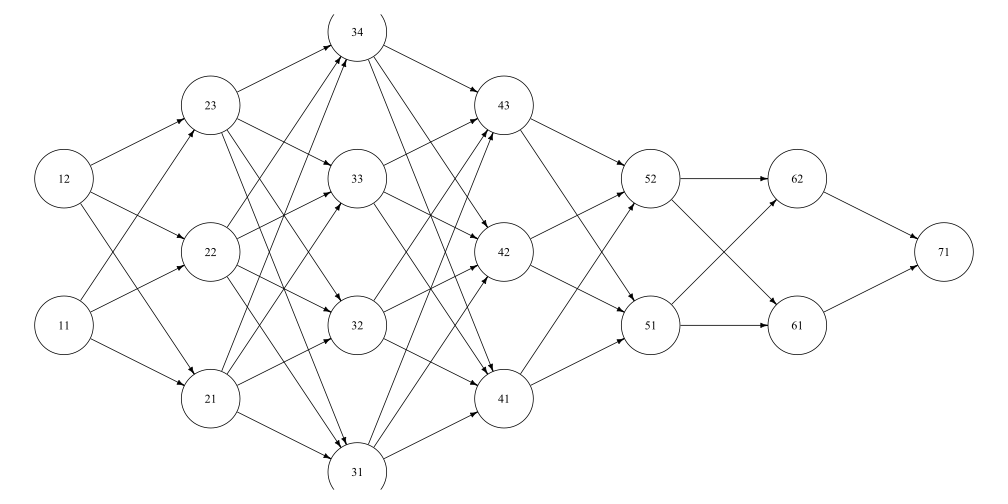
\includegraphics[trim={0 4.3cm 0 4.3cm}, width=\textwidth]{figures/nn.pdf}
  \caption{Neural network with four hidden layers}
  \label{fig:nn}
\end{figure}

A \textit{neural network} is a connected system of nodes and directed arcs, similar to a Bayesian network.
The differences between neural networks and Bayesian networks are that each node in a neural network consists of an activation function, a loss function, and an optimization algorithm, and each arc is assigned a weight based on its relative importance.

A \textit{deep feedforward neural network} is a neural network with an input layer, two or more hidden layers, and an output layer (Figure \ref{fig:nn}).
A deep feedforward neural network is comprised of many different functions, which approximate $\theta$ in the function $f(x;\theta)$ and form complex chains that map $x$ to $f(x;\theta)$.
Each chain is a function of the form $f_{i}(f_{i - 1}(f_{i - 2}(... (f_{i = 1}(x;\theta)))))$ where the maximum value of $i$ represents the depth of the network.
The output of the first hidden layer of the neural network, shown in Figure \ref{fig:nn}, is calculated using \ref{eq:nn1}.
%
\begin{equation}
  \label{eq:nn1}
  \left[
  \begin{matrix}
    x_{21} \\
    x_{22} \\
    x_{23} \\
  \end{matrix}
  \right] = g
  \left(
  \left[
  \begin{matrix}
    W_{10 \rightarrow 21} x_{10} + W_{11 \rightarrow 21} x_{11} + W_{12 \rightarrow 21} x_{12} \\
    W_{10 \rightarrow 22} x_{10} + W_{11 \rightarrow 22} x_{11} + W_{12 \rightarrow 22} x_{12} \\
    W_{10 \rightarrow 23} x_{10} + W_{11 \rightarrow 23} x_{11} + W_{12 \rightarrow 23} x_{12} \\
  \end{matrix}
  \right] + b_{1}
  \right)
\end{equation}

\noindent where \\
\indent $x_{ij} = $ output of neuron $ij$ \\
\indent $W_{ij \rightarrow (i + 1)k} = $ weight from the output of neuron $ij$ to the input of neuron $(i + 1)k$ \\
\indent $b_{i} = $ bias \\
\indent $g(x) = $ activation function \\

\noindent Similarly, the output of each hidden layer, shown in Figure \ref{fig:nn}, is calculated using \ref{eq:nn2}.
%
\begin{equation}
  \label{eq:nn2}
  \begin{split}
    &
    \left[
    \begin{matrix}
      x_{31} \\
      x_{32} \\
      x_{33} \\
      x_{34} \\
    \end{matrix}
    \right] = g
    \left(
    \left[
    \begin{matrix}
      W_{20 \rightarrow 31} x_{20} + W_{21 \rightarrow 31} x_{21} + W_{22 \rightarrow 31} x_{22} + W_{23 \rightarrow 31} x_{23} \\
      W_{20 \rightarrow 32} x_{20} + W_{21 \rightarrow 32} x_{21} + W_{22 \rightarrow 32} x_{22} + W_{23 \rightarrow 32} x_{23} \\
      W_{20 \rightarrow 33} x_{20} + W_{21 \rightarrow 33} x_{21} + W_{22 \rightarrow 33} x_{22} + W_{23 \rightarrow 33} x_{23} \\
      W_{20 \rightarrow 34} x_{20} + W_{21 \rightarrow 34} x_{21} + W_{22 \rightarrow 34} x_{22} + W_{23 \rightarrow 34} x_{23} \\
    \end{matrix}
    \right] + b_{2}
    \right) \\
    &
    \left[
    \begin{matrix}
      x_{41} \\
      x_{42} \\
      x_{43} \\
    \end{matrix}
    \right] = g
    \left(
    \left[
    \begin{matrix}
      W_{30 \rightarrow 41} x_{30} + W_{31 \rightarrow 41} x_{31} + W_{32 \rightarrow 41} x_{32} + W_{33 \rightarrow 41} x_{33} + W_{34 \rightarrow 41} x_{34} \\
      W_{30 \rightarrow 42} x_{30} + W_{31 \rightarrow 42} x_{31} + W_{32 \rightarrow 42} x_{32} + W_{33 \rightarrow 42} x_{33} + W_{34 \rightarrow 42} x_{34} \\
      W_{30 \rightarrow 43} x_{30} + W_{31 \rightarrow 43} x_{31} + W_{32 \rightarrow 43} x_{32} + W_{33 \rightarrow 43} x_{33} + W_{34 \rightarrow 43} x_{34} \\
    \end{matrix}
    \right] + b_{3}
    \right) \\
    &
    \left[
    \begin{matrix}
      x_{51} \\
      x_{52} \\
    \end{matrix}
    \right] = g
    \left(
    \left[
    \begin{matrix}
      W_{40 \rightarrow 51} x_{40} + W_{41 \rightarrow 51} x_{41} + W_{42 \rightarrow 51} x_{42} + W_{43 \rightarrow 51} x_{43} \\
      W_{40 \rightarrow 52} x_{40} + W_{41 \rightarrow 52} x_{41} + W_{42 \rightarrow 52} x_{42} + W_{43 \rightarrow 52} x_{43} \\
    \end{matrix}
    \right] + b_{4}
    \right)
  \end{split}
\end{equation}

\noindent The output of the last layer, shown in Figure \ref{fig:nn}, is calculated using \ref{eq:nn3}.
Unlike \ref{eq:nn1} and \ref{eq:nn2}, \ref{eq:nn3} uses a linear activation function, which is the same as having no activation function.
This allows the neural network to generate output that is positive or negative (Figure \ref{fig:relu}) \cite{goodfellow}.
%
\begin{equation}
  \label{eq:nn3}
  \left[
  \begin{matrix}
    x_{61}
  \end{matrix}
  \right] =
  \left[
  \begin{matrix}
    W_{50 \rightarrow 61} x_{50} + W_{51 \rightarrow 61} x_{51} + W_{52 \rightarrow 61} x_{52}
  \end{matrix}
  \right] + b_{5}
\end{equation}

\noindent Following \ref{eq:nn1}-\ref{eq:nn3} results in one forward pass of input through the neural network.
The vector output from \ref{eq:nn3} is then passed to a loss function, which for regression problems, is typically the \gls{mse}, shown in \ref{eq:mse1} \cite{chollet, goodfellow}.
%
\begin{equation}
  \label{eq:mse1}
  \mbox{MSE} = \frac{1}{n} \sum_{j = 1}^{n} (x_{observed_{j}} - x_{predicted_{j}})^2
\end{equation}

\noindent where \\
\indent $n = $ total number of variables that are observed or predicted \\
\indent $x = $ vector of observations or predictions \\

In this work, each neural network layer is densely (or fully) connected, and each hidden neuron uses a rectified linear unit activation function, which is a piecewise function that returns $x$ if $x > 0$ and 0 if $x \leq 0$ (Figure \ref{fig:relu}).

\vspace{+0.6cm}
\begin{figure}[H]
  \centering
  \includegraphics[scale=1]{figures/relu.png}
  \caption{Rectified linear unit (ReLU) activation function}
  \label{fig:relu}
\end{figure}

\noindent A simplified equation for a deep feedforward neural network with four hidden layers is shown in \ref{eq:nn4} \cite{goodfellow}.
%
\begin{equation}
  \label{eq:nn4}
  f(x; W, b) = W_{5}^{\top} \prod_{i = 1}^{4} \left( max \{ 0, W_{i}^{\top} x_{i} + b_{i} \} \right) + b_{5}
\end{equation}

\noindent where \\
\indent $W_{5}^{\top} + b_{5} = $ row vector mapping the last hidden layer to the output layer \\
\indent $max \{ 0, W_{i}^{\top} x_{i} + b_{i} \} = $ row vector mapping adjacent input and hidden layers \\

\noindent \ref{eq:mse1} is the general form of the \gls{mse} equation.
Substituting $x_{predicted_{i}}$ for the right side of \ref{eq:nn4} yields \ref{eq:mse2}.
%
\begin{equation}
  \label{eq:mse2}
  \mbox{MSE} = \frac{1}{n} \sum_{j = 1}^{n} \left( y_{j} - \left[ W_{5}^{\top} \prod_{i = 1}^{4} \left( max \{ 0, W_{i}^{\top} x_{i} + b_{i} \} \right) + b_{5} \right]_{j} \right)^{2}
\end{equation}

\noindent The output from the \gls{mse} loss function (\ref{eq:mse2}) is passed to the optimization algorithm, which updates parameters ($\theta$) by implementing the backpropagation algorithm \cite{goodfellow}.
The backpropagation algorithm is the backbone of a neural network and applies the chain rule to compute gradients (i.e., the vector of partial derivatives with respect to $\theta$ evaluated at time step \textit{i} \ref{alg:adamax}) and update parameters ($\theta$) \cite{goodfellow}.
These parameters ($\theta$) are also referred to as the weights ($W$) and biases ($b$) of the neural network in \ref{eq:nn1}-\ref{eq:nn4}.
In this work, the Adamax optimization algorithm (Algorithm \ref{alg:adamax}) is used to update parameters ($\theta$) \cite{kingma}.
Adamax is a variant of Adam (Algorithm \ref{alg:adam}) \cite{kingma} based on the exponentially weighted infinity norm, which takes the place of the bias-corrected first and second moment estimates \cite{kingma}.

\vspace{+0.6cm}
\begin{algorithm}[H]
  \centering
  \caption{Adamax optimization algorithm \cite{kingma}}
  \label{alg:adamax}
  \begin{algorithmic}
    \STATE \textbf{Require}: $\alpha = $ step size
    \STATE \textbf{Require}: $\beta_{1}, \beta_{2} \in \left[ 0, 1 \right) = $ exponential decay rates for the moment estimates
    \STATE \textbf{Require}: $f(x; \theta) = $ loss function with parameters $\theta$
    \STATE \textbf{Require}: $\theta_{0} = $ initial parameter vector
    \STATE $m_{0} \leftarrow 0$ (initialize first moment vector)
    \STATE $u_{0} \leftarrow 0$ (initialize exponentially weighted infinity norm)
    \STATE $i \leftarrow 0$ (initialize first iteration)
    \STATE \textbf{while} $\theta_{i}$ not converged \textbf{do}
    \STATE \hspace{\algorithmicindent} $i \leftarrow i + 1$
    \STATE \hspace{\algorithmicindent} $g_{i} \leftarrow \bigtriangledown_{\theta} f_{i} (\theta_{i - 1})$ (get gradients from loss function at time step $i$)
    \STATE \hspace{\algorithmicindent} $m_{i} \leftarrow \beta_{1} \cdot m_{i - 1} + (1 - \beta_{1}) \cdot g_{i}$ (update biased first moment estimate)
    \STATE \hspace{\algorithmicindent} $u_{i} \leftarrow max(\beta_{2} \cdot u_{t - 1}, |g_{i}|)$ (update exponentially weighted infinity norm)
    \STATE \hspace{\algorithmicindent} $\theta_{i} \leftarrow \theta_{t - 1} - (\alpha / (1 - \beta_{1}^{i})) \cdot m_{i} / u_{i}$ (update parameters)
    \STATE \textbf{return} $\theta_{i}$
  \end{algorithmic}
\end{algorithm}

\vspace{+0.6cm}
\begin{algorithm}[H]
  \centering
  \caption{Adam optimization algorithm \cite{kingma}}
  \label{alg:adam}
  \begin{algorithmic}
    \STATE \textbf{Require}: $\alpha = $ step size
    \STATE \textbf{Require}: $\beta_{1}, \beta_{2} \in \left[ 0, 1 \right) = $ exponential decay rates for the moment estimates
    \STATE \textbf{Require}: $f(x; \theta) = $ loss function with parameters $\theta$
    \STATE \textbf{Require}: $\theta_{0} = $ initial parameter vector
    \STATE $m_{0} \leftarrow 0$ (initialize first moment vector)
    \STATE $v_{0} \leftarrow 0$ (initialize second moment vector)
    \STATE $i \leftarrow 0$ (initialize first iteration)
    \STATE \textbf{while} $\theta_{i}$ not converged \textbf{do}
    \STATE \hspace{\algorithmicindent} $i \leftarrow i + 1$
    \STATE \hspace{\algorithmicindent} $g_{i} \leftarrow \bigtriangledown_{\theta} f_{i} (\theta_{i - 1})$ (get gradients from loss function at time step $i$)
    \STATE \hspace{\algorithmicindent} $m_{i} \leftarrow \beta_{1} \cdot m_{i - 1} + (1 - \beta_{1}) \cdot g_{i}$ (update biased first moment estimate)
    \STATE \hspace{\algorithmicindent} $v_{i} \leftarrow \beta_{2} \cdot v_{i - 1} + (1 - \beta_{2}) \cdot g_{i}^{2}$ (update biased second moment estimate)
    \STATE \hspace{\algorithmicindent} $\hat m_{i} \leftarrow m_{i} / (1 - \beta_{1}^{i})$ (calculate bias-corrected first moment estimate)
    \STATE \hspace{\algorithmicindent} $\hat v_{i} \leftarrow v_{i} / (1 - \beta_{2}^{i})$ (calculate bias-corrected second moment estimate)
    \STATE \hspace{\algorithmicindent} $\theta_{i} \leftarrow \theta_{i - 1} - \alpha \cdot \hat m_{i} / (\sqrt{\hat v_{i}} + \epsilon)$ (update parameters)
    \STATE \textbf{return} $\theta_{i}$
  \end{algorithmic}
\end{algorithm}

  % !TEX root = ../dissertation.tex
% !TEX root = ../tex/bn.tex

\chapter{Bayesian Network}

The Bayesian network, shown in Figure \ref{fig:bn2}, is comprised of 8 nodes and 13 arcs, which represent fissionable material operations (\textit{op}), criticality controls (\textit{ctrl}), and parameters that affect nuclear criticality \cite{mclaughlin}.
%
\begin{figure}[H]
  \centering
  \includegraphics[trim={1cm 4.8cm 1cm 4.8cm}, width=\textwidth]{figures/bn.pdf}
  \caption{Bayesian network}
  \label{fig:bn2}
\end{figure}

The \textit{bnlearn} \cite{bnlearn} and \textit{igraph} \cite{igraph} software packages were used to build the Bayesian network and randomly sample parameters using the forward sampling algorithm (Algorithm \ref{alg:bn-fwd}).
Fissionable material operations are divided into six categories (Table \ref{table:op1}), based on safety plans and work control documents that describe each operation, as well as the criticality controls that apply to them.
Criticality controls in Building 332 consist of standardized sets of controls that are analyzed and approved for individual fissionable material operations.
Each set of controls has a single letter designation and consists of administrative limits on plutonium mass, form, moderation, and reflection (Table \ref{table:ctrl1}).
%
\begin{table}
  \caption{Fissionable material operations in Building 332}
  \label{table:op1}
  \renewcommand\arraystretch{1.5}
  \begin{center}
    \begin{tabular}{|l p{10.16cm}|}
      \hline
      operation    & description \\
      \hline
      large sample & operations with $\geq$ 65 g of plutonium \\
      machining    & operations with a drill press, grinder, lathe, mill, saw, or other cutting equipment \\
      metallurgy   & operations with a casting furnace or other heating equipment \\ 
      small sample & operations with $<$ 65 g of plutonium \\
      solution     & operations with liquids \\
      waste        & operations with radioactive waste \\
      \hline
    \end{tabular}
  \end{center}
\end{table}

\begin{table}
  \caption{Conditional probability table for fissionable material operations in Building 332}
  \label{table:op2}
  \renewcommand\arraystretch{1.5}
  \begin{center}
    \begin{tabular}{|c c c c c c|}
      \hline
      large sample & machining & metallurgy & small sample & solution & waste \\
      \hline
      0.3421       & 0.0789    & 0.1316     & 0.3158       & 0.1053   & 0.0263 \\
      \hline
    \end{tabular}
  \end{center}
\end{table}

\begin{table}
  \caption{Criticality controls in Building 332}
  \label{table:ctrl1}
  \renewcommand\arraystretch{1.5}
  \begin{center}
    \begin{tabular}{|c l l l l|}
      \hline
      condition & mass          & form               & moderation                      & reflection \\
      \hline
      A         & $\leq$ 65 g   &                    & no D$_{2}$O                     & \\
      B         & $\leq$ 220 g  &                    & H/X $\leq$ H$_{2}$O, $\leq$ 4 L & no Be/C/D$_{2}$O, $\leq$ 2 in \\
      C         & $\leq$ 1200 g &                    & $\leq$ 2.5 L                    & none \\
      D         & $\leq$ 2500 g &                    & $\leq$ 1 L                      & $\leq$ 2 L, $\leq$ 0.25 in \\
      E         & $\leq$ 2500 g &                    & none                            & $\leq$ 0.25 in \\
      M         & $\leq$ 4000 g & $\leq$ 500 g fines & $\leq$ 1 in, $\leq$ 4 L         & $\leq$ 0.3 in \\
      P         & $\leq$ 300 g  &                    & no liquids                      & $\leq$ 3.5 kg Be/C \\
      \hline
    \end{tabular}
  \end{center}
\end{table}

Most fissionable material operations have two to five sets of criticality controls.
However, only one set of criticality controls can be active at each workstation.
For example, a fissile material handler can use \textit{Condition A} at one workstation, and then switch to \textit{Condition E} if the operation requires them to move $>$ 65 grams of plutonium into the workstation.
To facilitate this move, the handler is required to ensure that the more restrictive moderator and reflector limits of \textit{Condition E} are met prior to switching from \textit{Condition A}.
The conditional probability table for each set of criticality controls (\textit{ctrl}), shown in Table \ref{table:ctrl2}, is derived from walkthrough forms, which nuclear engineers use to document active criticality controls at each workstation in the facility.

The parameters that affect nuclear criticality in Building 332 are shown in Table \ref{table:param}.
These parameters link fissionable material operations (Table \ref{table:op1}) and criticality controls (Table \ref{table:ctrl2}) to the bottom-tier Bayesian network parameters, shown in Figure \ref{fig:bn2}.
Spherical geometry and surrogate materials (Table \ref{table:param}) were selected to conservatively bound the physics of a process criticality accident.
Spherical geometry is used because a sphere has the lowest surface area-to-volume ratio of any object, which reduces neutron leakage and therefore increases $k_{eff}$ \cite{knief}.
Water is used instead of organic and inorganic liquids because it provides superior moderation and reflection, which also increases $k_{eff}$ \cite{knief}.
Polyethylene is similarly used instead of rubber, filter paper, foam, thermocouple insulation, and plastic.
Magnesium oxide (MgO) is included in Table \ref{table:param} because it is commonly used in crucibles.
Sepiolite is included because it is used to downblend plutonium oxide and absorb liquids in waste.
Other materials, such as aluminum, beryllium, depleted uranium ($^{238}$U), graphite (C), and 304 stainless steel are included because they are used in experiments or are integral to gloveboxes and process equipment.
%
\begin{table}
  \caption{Conditional probability table for criticality controls in Building 332}
  \label{table:ctrl2}
  \renewcommand\arraystretch{1.5}
  \begin{center}
    \begin{tabular}{|c l l l l l l|}
      \hline
      condition & large sample & machining & metallurgy & small sample & solution & waste \\
      \hline
      A         & 0.5714       & 0.1538    & 0.6154     & 0.9375       & 1        & 0.5 \\
      B         & 0.0286       & 0         & 0.0769     & 0.0625       & 0        & 0 \\
      C         & 0.0286       & 0         & 0          & 0            & 0        & 0 \\
      D         & 0.1714       & 0         & 0          & 0            & 0        & 0 \\
      E         & 0.0857       & 0         & 0.3077     & 0            & 0        & 0 \\
      M         & 0.1143       & 0.8462    & 0          & 0            & 0        & 0 \\
      P         & 0            & 0         & 0          & 0            & 0        & 0.5 \\
      \hline
    \end{tabular}
  \end{center}
\end{table}

\begin{table}
  \caption{Parameters that affect nuclear criticality in Building 332}
  \label{table:param}
  \renewcommand\arraystretch{1.5}
  \begin{center}
    \begin{tabular}{|l l|}
      \hline
      parameter                          & description \\
      \hline
      \textit{mass}                      & grams of plutonium (95\% $^{239}$Pu, 5\% $^{240}$Pu by weight) \\
      \textit{form}                      & plutonium in the form of alpha-phase metal or oxide (PuO$_{2}$) \\
      moderator (\textit{mod})           & MgO, CH$_{2}$, sepiolite, H$_{2}$O, or none \\
      radius (\textit{rad})              & radius of sphere (in or cm) \\
      reflector (\textit{ref})           & Al, Be, $^{238}$U, C, Pb, MgO, CH$_{2}$, \gls{ss304}, H$_{2}$O, or none \\
      reflector thickness (\textit{thk}) & reflector thickness (in or cm) \\
      \textit{shape}                     & sphere \\
      volume (\textit{vol})              & volume of sphere (cm$^{3}$) \\
      concentration (\textit{conc})      & concentration of plutonium in solution (g/cm$^{3}$) \\
      \hline
    \end{tabular}
  \end{center}
\end{table}

\section{Fitting Probability Distributions}

The probability tables for operations (\textit{op}), controls (\textit{ctrl}), \textit{form}, \textit{moderator}, and \textit{reflector} were populated directly from unclassified computer records and waste parcel cards.
The probability tables for \textit{mass}, \textit{radius}, and \textit{reflector thickness}, however, are based on truncated probability distributions (\ref{eq:gamma}-\ref{eq:weibull}) that were fit to incomplete data using the maximum likelihood estimation method \cite{d'agostino}.
Truncated gamma and normal distributions were selected because they are commonly used distributions that fit the data reasonably well (Table \ref{table:test}).
Truncated log-normal and Weibull distributions were selected because they are heavy right-tailed distributions, which increases the probability of generating random samples that result in a criticality accident.
The probability density functions of these distributions are shown in \ref{eq:gamma}-\ref{eq:weibull} \cite{devore}.
%
\begin{equation}
  \label{eq:gamma}
    \mbox{gamma distribution} \quad f(x; \alpha, \beta) = \frac{\beta^{\alpha}x^{\alpha - 1}e^{-\beta x}}{\Gamma(\alpha)} \quad x, \alpha, \beta > 0
\end{equation}

\begin{equation}
  \label{eq:normal}
  \mbox{normal distribution} \quad f(x; \mu, \sigma^{2}) = \frac{1}{\sqrt{2 \pi \sigma^{2}}} e^{\frac{(x - \mu)^{2}}{2 \sigma^{2}}}
\end{equation}

\begin{equation}
  \label{eq:log-normal}
  \mbox{log-normal distribution} \quad f(x; \mu, \sigma) = \frac{1}{\sqrt{2 \pi} \sigma x} e^{\frac{(\ln x - \mu)^{2}}{2 \sigma^{2}}}
\end{equation}

\begin{equation}
  \label{eq:weibull}
  \mbox{Weibull distribution} \quad f(x; \lambda, k) =
  \begin{cases}
    \frac{k}{\lambda} (\frac{x}{\lambda})^{k - 1} e^{-(\frac{x}{\lambda})^{k}} & x \geq 0 \\
    0 & x < 0
  \end{cases}
\end{equation}
\\
\noindent The maximum likelihood estimators are derived from the likelihood function, shown in \ref{eq:mle1}, where $X_{1}, ..., X_{n}$ are independent and indentically distributed random variables from a population with a probability density function $f(x | \theta_{1}, ..., \theta_{k}$.
%
\begin{equation}
  \label{eq:mle1}
  L(\theta | x) = L(\theta_{1}, ..., \theta_{k} | x_{1}, ..., x_{n}) = \prod_{i = 1}^{n} f(x_{i} | \theta_{1}, ..., \theta_{k})
\end{equation}

\noindent 

Once the probability distributions were fit to the data, they were trucated by selecting a conservatively large upper limit for each variable, removing values beyond the limits, and then normalizing the remaining values so that each row in the conditional probability table sums to one.
Kolmogorov-Smirnov \cite{massey}, Cram\'{e}r-von Mises, \cite{cramer}, and Anderson-Darling \cite{anderson} tests were also performed to determine the goodness of fit for each probability distribution.
The general formulas for these test statistics are shown in \ref{eq:ks}-\ref{eq:ad} \cite{anderson,cramer,massey}, where $F_{n}$ is the empirical distribution function and $F_{0}$ is the fitted cumulative distribution function.
The test statistics were calculated using the \textit{fitdistrplus} \cite{fitdistrplus} software package and compared to the critical values in R.B. D'Agostino and M.A. Stephens \cite{d'agostino}.
%
\begin{equation}
  \label{eq:ks}
  \mbox{Kolmogorov-Smirnov test statistic} \quad D = \sup_{x} | F_{n}(x) - F_{0}(x) |
\end{equation}
\vspace{+0.4cm}
\begin{equation}
  \label{eq:cvm}
  \mbox{Cram\'{e}r-von Mises test statistic} \quad W_{n}^{2} = n \int_{-\infty}^{\infty} (F_{n}(x) - F_{0}(x))^2 dF_{0}(x)
\end{equation}

\begin{equation}
  \label{eq:ad}
  \mbox{Anderson-Darling test statistic} \quad A_{n}^{2} = n \int_{-\infty}^{\infty} \frac{(F_{n}(x) - F_{0}(x))^2}{F_{0}(x)(1 - F_{0}(x))}
\end{equation}
\vspace{+0.4cm}
An example set of truncated gamma distributions and quantile-quantile (Q-Q) plots for the 65-gram \textit{Condition A} mass limit are shown in Figures \ref{fig:gamma} and \ref{fig:qq}.
Histograms of Kolmogorov-Smirnov \cite{massey}, Cram\'{e}r-von Mises, \cite{cramer}, and Anderson-Darling \cite{anderson} test statistics are shown in Figure \ref{fig:hist} and Table \ref{table:test}.
The critical values of these test statistics (Table \ref{table:test}) correspond to a significance level of $\alpha = 0.05$ with $n = 500$ samples \cite{d'agostino}.
%
\begin{figure}
  \centering
  \includegraphics[width=\textwidth]{figures/gamma.png}
  \caption{Truncated gamma distributions for 65-gram mass limit}
  \label{fig:gamma}
  \vspace{+1.1cm}
  \includegraphics[width=\textwidth]{figures/gamma-qq.png}
  \caption{Q-Q plots of truncated gamma distributions for 65-gram mass limit}
  \label{fig:qq}
\end{figure}

\begin{figure}[H]
  \centering
  \includegraphics[width=\textwidth]{figures/hist.png}
  \caption{Histograms of test statistics}
  \label{fig:hist}
\end{figure}

\begin{table}
  \caption{Test statistics}
  \label{table:test}
  \renewcommand\arraystretch{1.5}
  \begin{center}
    \begin{tabular}{|l|c c|c c|c c|}
      \multicolumn{1}{c}{} & \multicolumn{2}{c}{KS test statistic} & \multicolumn{2}{c}{CVM test statistic} & \multicolumn{2}{c}{AD test statistic} \\
      \hline
      distribution         & mean  & range                      & mean  & range                       & mean  & range \\
      \hline
      gamma                & 0.105 & 0.052-0.305                & 0.626 & 0.056-1.339                 & 3.704 & 0.333-7.909 \\
      normal               & 0.083 & 0.039-0.278                & 0.411 & 0.038-0.883                 & 2.810 & 0.301-5.787 \\
      log-normal           & 0.148 & 0.089-0.313                & 1.663 & 0.041-2.796                 & 9.870 & 0.271-16.348 \\
      Weibull              & 0.081 & 0.029-0.307                & 0.305 & 0.020-0.802                 & 2.126 & 0.158-5.581 \\
      \hline
      critical value       & \multicolumn{2}{c|}{0.061}         & \multicolumn{2}{c|}{0.220}          & \multicolumn{2}{c|}{0.751-0.795} \\
      \hline
    \end{tabular}
  \end{center}
\end{table}

The results shown in Table \ref{table:test} indicate that the test statistics for the truncated gamma, normal, and Weibull distributions fit the data slightly better than the truncated log-normal distributions---although this is by no means a definitive assessment of each fit.
The purpose of calculating these test statistics is to document the goodness of fit, which is commonly used in conjunction with graphical checks of Q-Q plots (Figure \ref{fig:qq}) to validate risk models in the nuclear industry.

\section{Generating Random Samples}

The Bayesian network forward sampling algorithm (\ref{alg:bn-fwd}) is used to generate random samples, which are passed to the neural network metamodel.

  % !TEX root = ../dissertation.tex
% !TEX root = ../tex/nn-metamodel.tex

\chapter{Neural Network Metamodel}

The neural network metamodel is comprised of 10 neural neural networks that were built using the \textit{Keras} \cite{keras} and \textit{TensorFlow} \cite{tensorflow} software packages.
The main benefit of using a neural network metamodel is that it can generate predictions in less time than it takes MCNP to perform the same number of calculations. % add reference to figure/table here
This is especially beneficial if millions (or even billions) of predictions are needed to estimate process criticality accident risk and reduce the variance ($v$) of the risk estimate to an acceptable (low) value (\ref{eq:var}).
%
\begin{equation}
  \label{eq:var}
  v = \frac{1}{n} \sum_{i = 1}^{n}(x_{i} - \bar{x})^{2}
\end{equation}

\noindent where \\
\indent $v = $ variance of the risk estimate \\
\indent $n = $ number of samples \\
\indent $x_{i} = $ risk estimate (e.g., 1e-07 accidents/year) \\
\indent $\bar{x} = $ mean risk estimate \\

\noindent Each of the 10 neural networks has the same structure, which consists of one input layer, six hidden layers, and one output layer.
The input layer has 28 neurons that correspond to the Bayesian network parameters, shown in Table \ref{table:param}, and the output layer has one neuron that corresponds to $k_{eff}$.
The six hidden layers have the following number of neurons in each layer: 8192-256-256-256-256-16.
The number of hidden layers and the number of neurons in each hidden layer were determined using a manual training process, described in the next sections.

\section{Preparing Data}

Each neural network was trained using a 64-16-20 data split, based on the parameters shown in Table \ref{table:output1}.
This was done by setting aside 20\% of the 1,542,792 output files for testing, and splitting the other 80\% into two groups of 64\% for training and 16\% for cross-validation.
This is also sometimes called an 80-20 data split because 64\% is 80\% of 80\% of the 1,542,792 output files, and 16\% is 20\% of 80\%.
%
\begin{table}
  \caption{Training parameters based on 1,542,792 MCNP output files}
  \label{table:output1}
  \renewcommand\arraystretch{1.5}
  \begin{center}
    \begin{tabular}{|l l|}
      \hline
      parameter                          & description \\
      \hline
      \textit{mass}                      & 0-4 kg of Pu in 25 g increments \\
      \textit{form}                      & Pu (19.86 g/cm$^{3}$) or PuO$_{2}$ (11.5 g/cm$^{3}$) \\
      moderator (\textit{mod})           & MgO, CH$_{2}$, sepiolite, H$_{2}$O, or none \\
      radius (\textit{rad})              & 0-18 inches in 1-inch increments \\
      reflector (\textit{ref})           & Al, Be, $^{238}$U, C, Pb, MgO, CH$_{2}$, SS304, H$_{2}$O, or none \\
      reflector thickness (\textit{thk}) & 0-6 inches in 1-inch increments \\
      \textit{shape}                     & sphere \\
      volume (\textit{vol})              & volume of sphere (cm$^{3}$) \\
      concentration (\textit{conc})      & concentration of Pu in solution (g/cm$^{3}$) \\
      \hline
    \end{tabular}
  \end{center}
\end{table}

A much smaller set of output files (Table \ref{table:output2}) was initially used because each neural network took several hours to train, and it wasn't feasible to spend hundreds of hours training a neural network metamodel.
Later on, it was determined that the accuracy of neural networks could be improved by training for fewer epochs (i.e., fewer passes of training data) on a larger dataset. % add reference to figure/table here
The increments and upper limits of the discrete parameters, shown in Tables \ref{table:output1} and \ref{table:output2}, were selected based on the rationale discussed previously, as well as the total amount of fissionable material that is allowed in Building 332, a Security Category III nuclear facility (\ref{ch:doe-o-474}).
The parameters, shown in Tables \ref{table:output1} and \ref{table:output2}, and the \textit{Grid} (\ref{sec:grid}) and \textit{Build} (\ref{sec:build}) functions were used to build and run the MCNP input decks on Quartz, a supercomputer at Lawrence Livermore National Laboratory (Figure \ref{fig:quartz}).
Once the MCNP input decks were run, data from the output files was extracted, processed, and written to comma-separated values (CSV) and RData files, using the \textit{Tabulate} (\ref{sec:tabulate}) and \textit{Split} (\ref{sec:split}) functions.
%
\begin{table}
  \caption{Training parameters based on 202,786 MCNP output files}
  \label{table:output2}
  \renewcommand\arraystretch{1.5}
  \begin{center}
    \begin{tabular}{|l l|}
      \hline
      parameter                          & description \\
      \hline
      \textit{mass}                      & 0-2 kg of Pu in 50 g increments \\
      \textit{form}                      & Pu (19.86 g/cm$^{3}$) or PuO$_{2}$ (11.5 g/cm$^{3}$) \\
      moderator (\textit{mod})           & MgO, CH$_{2}$, sepiolite, H$_{2}$O, or none \\
      radius (\textit{rad})              & 0-18 inches in 1-inch increments \\
      reflector (\textit{ref})           & Al, Be, $^{238}$U, C, Pb, MgO, CH$_{2}$, SS304, H$_{2}$O, or none \\
      reflector thickness (\textit{thk}) & 0-3 inches in 1-inch increments \\
      \textit{shape}                     & sphere \\
      volume (\textit{vol})              & volume of sphere (cm$^{3}$) \\
      concentration (\textit{conc})      & concentration of Pu in solution (g/cm$^{3}$) \\
      \hline
    \end{tabular}
  \end{center}
\end{table}

\begin{figure}
  \centering
  \includegraphics[trim={1cm 5cm 6cm 3cm}, clip, width=\textwidth]{figures/quartz.jpg}
  \caption{Quartz supercomputer at Lawrence Livermore National Laboratory}
  \label{fig:quartz}
\end{figure}

The training data was scaled by calculating the column-wise mean and standard deviation of each discrete variable, subtracting each mean from its corresponding column, and then dividing each column by its corresponding standard deviation.
These last two steps were repeated for the test data using the means and standard deviations from the training data.
The training and test data were then one-hot-encoded using the \textit{dummyVars} function in the \textit{caret} \cite{caret} software package, which converts categorical variables into multi-column dummy variables, where membership within each sub-category is 0 or 1.
The purpose of scaling and one-hot-encoding data was to improve the initial parameter ($\theta$) updates of the neural network \cite{chollet}, and minimize bias towards individual training parameters (Table \ref{table:output2}).

\section{Training Neural Networks}

Each neural network was initially trained for 1,500 epochs using a "mini-batch" training approach \cite{goodfellow}, which consists of splitting the training data into smaller batches of 8,192, computing gradients using \gls{mse} (\ref{eq:mse1}), and updating parameters ($\theta$) after each batch.
Then, each neural network was trained for an additional 150 epochs, and the model was saved as a separate HDF5 file after each epoch.
Lastly, each neural network was evaluated by comparing the sum of mean absolute errors (\ref{eq:mae}) on training and cross-validation data for the last 150 epochs (Figures \ref{fig:train1} and \ref{fig:train2}).
The neural network with the lowest sum of mean absolute errors was selected as the baseline for the neural network metamodel.
To correct for possible bias towards cross-validation data (i.e., the smaller dataset), the weighted averages were also compared (Figures \ref{fig:train-wt1} and \ref{fig:train-wt2}).
Although the sums and weighted averages differ slightly, the selected neural network has the lowest sum and weighted average of mean absolute errors on training and cross-validation data, so there is no change in outcome (Figures \ref{fig:train1}-\ref{fig:train-wt2}).
%
\begin{equation}
  \label{eq:mae}
  \mbox{mean absolute error (MAE)} = \frac{1}{n} \sum_{i = 1}^{n} | x_{observed_{i}} - x_{predicted_{i}} |
\end{equation}

\begin{figure}
  \centering
  \includegraphics[width=\textwidth]{figures/train1.png}
  \caption{Sum of mean absolute errors on training and cross-validation data}
  \label{fig:train1}
  \vspace{+1.1cm}
  \includegraphics[width=\textwidth]{figures/train2.png}
  \caption{Sum of mean absolute errors on training and cross-validation data}
  \label{fig:train2}
\end{figure}

\begin{figure}
  \centering
  \includegraphics[width=\textwidth]{figures/train-wt1.png}
  \caption{Weighted average of mean absolute errors on training and cross-validation data}
  \label{fig:train-wt1}
  \vspace{+1.1cm}
  \includegraphics[width=\textwidth]{figures/train-wt2.png}
  \caption{Weighted average of mean absolute errors on training and cross-validation data}
  \label{fig:train-wt2}
\end{figure}

\subsection{Applying a Sum of Squared Errors Loss Function}

The \gls{mse} loss function (\ref{eq:mse1}) was initially used to train each neural network.
The reason it was used is because nearly all journal articles, preprints
After reading more about loss functions in \textit{The Theory of Point Estimation} \cite{lehmann} and other books \cite{bertsekas,devore,kuhn}, and then failing to find any relevant journal articles or preprints on why MSE is  
Later on, the sum of squared errors loss function (\ref{eq:sse}) was tested, and it was found to outperform the more commonly used \gls{mse} loss function \cite{chollet,goodfellow}.
This section discusses why the sum of squared errors loss function (\ref{eq:sse}) is better, and provides empirical evidence and code to support this claim.
%
\begin{equation}
  \label{eq:sse}
  \mbox{sum of squared errors (SSE)} = \sum_{i = 1}^{n} (x_{observed_{i}} - x_{predicted_{i}})^{2}
\end{equation}

\noindent When a neural network is trained in batches, the number of samples in the last batch is calculated using \textit{n} mod \textit{b}, where \textit{n} is the number of training samples and \textit{b} is batch size.
Typically, this calculation results in a smaller last batch, except in cases where the number of training samples is evenly divisible by batch size.
A smaller last batch isn't a problem by itself, but when the \gls{mse} loss function (\ref{eq:mse1}) is used, the computed gradients are divided by the number of samples in each batch.
This causes the samples in the last batch to be weighted more heavily than all other samples, which causes parameter ($\theta$) updates to become more sensitive to the computed gradients of the last batch.

The effect the last batch has on training stability and overall performance is highly dependent on the optimization algorithm that is used.
A portion of the Adamax optimization algorithm (Algorithm \ref{alg:adamax}) is reproduced in Algorithm \ref{alg:while}, as it is implemented in the neural network metamodel (\ref{sec:nn}, \ref{sec:model}).

\vspace{+0.6cm}
\begin{algorithm}[H]
  \centering
  \caption{Adamax optimization algorithm \textbf{while} loop \cite{kingma}}
  \label{alg:while}
  \begin{algorithmic}
    \STATE \textbf{while} $\theta_{i}$ not converged \textbf{do}
    \STATE \hspace{\algorithmicindent} $i \leftarrow i + 1$
    \STATE \hspace{\algorithmicindent} $g_{i} \leftarrow \bigtriangledown_{\theta} f_{i} (\theta_{i - 1})$ (get gradients from loss function at time step $i$)
    \STATE \hspace{\algorithmicindent} $m_{i} \leftarrow 0.9 \cdot m_{i - 1} + (1 - 0.9) \cdot g_{i}$ (update biased first moment estimate)
    \STATE \hspace{\algorithmicindent} $u_{i} \leftarrow max(0.999 \cdot u_{t - 1}, |g_{i}|)$ (update exponentially weighted infinity norm)
    \STATE \hspace{\algorithmicindent} $\theta_{i} \leftarrow \theta_{t - 1} - (\alpha / (1 - 0.9^{i})) \cdot m_{i} / u_{i}$ (update parameters)
    \STATE \textbf{return} $\theta_{i}$
  \end{algorithmic}
\end{algorithm}

$\beta_{1}$ and $\beta_{2}$ are set to their default values of 0.9 and 0.999, respectively \cite{kingma}.
Under certain circumstances, it might make sense to subsitute each loss function into Algorithm \ref{alg:while} and apply the backpropagation algorithm \cite{goodfellow}.
However, since MSE and SSE are nearly the same, it is much easier to just examine the effect that the leading $\frac{1}{n}$ term (\ref{eq:mse1}) has on the parameter ($\theta$) updates.
The following code was written to perform pseudo parameter ($\theta$) updates under a relatively simple set of assumptions.

% -----------------------
% -----------------------
% -----------------------

The selected neural network was tested using several different optimization algorithms (Figure \ref{fig:opt}) that are available in \textit{TensorFlow} \cite{tensorflow} and other deep learning software packages.
Adamax \cite{kingma} outperformed all other optimization algorithms, as indicated by having the lowest sum of mean absolute errors on training and cross-validation data (Figure \ref{fig:opt}).
The Adamax optimization algorithm was also tested by varying the learning rate ($\alpha$), which is a scaling factor that controls how much the parameters ($\theta$) are updated during training (Figure \ref{fig:lr}).
The default Adamax learning rate is set to 0.002 \cite{tensorflow,chollet,kingma}.
%
\begin{figure}
  \centering
  \includegraphics[width=\textwidth]{figures/opt.png}
  \caption{Training the selected neural network using different optimization algorithms}
  \label{fig:opt}
\end{figure}

\begin{figure}
  \centering
  \includegraphics[width=\textwidth]{figures/lr.png}
  \caption{Training the selected neural network using different learning rates}
  \label{fig:lr}
\end{figure}

When the Adamax learning rate is set to 0.00075, the training error lowers to 1.9e-04, and the cross-validation error remains at 3.4e-04 (Figure \ref{fig:lr}).
As a result, the learning rate was set to 0.00075 to allow for more gradual parameter ($\theta$) updates.
20 neural networks were trained using this learning rate, and the results are plotted and shown in Figures \ref{fig:model}, \ref{fig:remodel}, and \ref{fig:model1}-\ref{fig:model20}.
%
\begin{figure}
  \centering
  \includegraphics[width=\textwidth]{figures/model.png}
  \caption{Training the selected neural network for 1,500 epochs}
  \label{fig:model}
  \vspace{+1.1cm}
  \includegraphics[width=\textwidth]{figures/remodel.png}
  \caption{Training the selected neural network for an additional 150 epochs}
  \label{fig:remodel}
\end{figure}

\section{Model Averaging}

The purpose of using more than one neural network is to reduce generalization error, which is the expected error on new input [41].
This was done by training 50 neural networks separately and then averaging the results of predicted keff values for the test data, which consists of 26,593 output files the neural networks have never seen.
The idea behind this technique, known as model averaging, is that each neural network in the ensemble metamodel will not make the same errors on test data [41].
The expected squared error of the ensemble metamodel, taken from Goodfellow, et al., [41] is shown in Eq. 10 for a set of n regression models with errors % (ϵi) that are drawn from a zero-mean multivariate distribution with variances E[ϵ_i ]=v and covariances E[〖ϵ_i ϵ〗_j ]=c.

If the errors are perfectly correlated, then c = v, and the expected squared error of the ensemble metamodel reduces to v [41].
Conversely, if the errors are perfectly uncorrelated, then c = 0, and the expected squared error reduces to v/n [41].
The ensemble metamodel test errors are plotted and shown in Fig. 14.

  % !TEX root = ../dissertation.tex
% !TEX root = ../tex/risk.tex

\chapter{Estimating Process Criticality Accident Risk}

% -------
% Results
% -------

\section{Results}

As expected, the results shown in Fig. 14 indicate that the test errors are partially correlated, as indicated by a decrease in test error as the number of neural networks in the ensemble metamodel increases.
These results also indicate that setting the learning rate to a value that corresponds to a lower training error allows the ensemble metamodel to asymptotically approach this lower value (Fig. 14).
Based on these results, it was determined that 10-20 neural networks would likely be enough to minimize the test error on the larger test data set (Table 6) without significantly extending the time it takes to train the ensemble metamodel.
An ensemble metamodel, comprised of 10 neural networks, was re-trained on 1,584,973 output files.
To accommodate the larger data set, batch size was increased to 32,768 output files.
The ensemble metamodel test errors are plotted and shown in Fig. 15, for a test data set that consists of 316,993 output files.

The test errors shown in Fig. 15 are slightly higher than previous test errors (Fig. 14), but low enough to forego further training and optimization.
These test errors were re-plotted to show the variation in individual output files (Fig. 16).

As shown in Fig. 16, the test errors become slightly more diffuse, but with fewer outliers, as keff increases.
The keff standard deviations of all 1,584,973 output files were plotted (Fig. 17) to summarize the keff standard deviations and show that test errors (Fig. 16) follow a similar trend.

The average ensemble metamodel test error is 2.74e-04 (Fig. 15), which is very close to the average standard deviation of 2.97e-04 (Fig. 17).
Even though these results are comparable, there are hundreds of outliers, including several that are 5-10 times larger than 2.74e-04.
Based on the results shown in Fig. 15 and Fig. 16, it is reasonable to conclude that the ensemble metamodel predicts keff to within % ± 0.02 of the keff that is calculated using MCNP6.2 [15] and ENDF/B-VII.1 nuclear data [17].

Now that the ensemble metamodel has been validated against MCNP6.2 [15] and ENDF/B-VII.1 nuclear data [17], it can be combined with the Bayesian network and used to estimate process criticality accident risk.
A preliminary estimate was performed by fitting gamma distributions to the data and running 1 million simulations (Fig. 18).

The results shown in Fig. 18 indicate that the hybrid risk model fails to predict a process criticality accident at a frequency % ≥ 1e-06 accidents per year.
However, since there are outliers, an additional 10 to 100 million simulations were run (Fig. 19, Fig. 20).

The results shown in Fig. 19 and Fig. 20 indicate that the risk of a process criticality accident in Building 332 is estimated to be 1e-07 accidents per year, based on the number of points above the upper subcritical limit.
This estimate has corresponding critical masses of approximately 600-730 grams of plutonium (95\% 239Pu, 5\% 240Pu by weight), which are very similar to 3 of the 7 spherical plutonium critical masses associated with historical process criticality accidents [1].
Additional estimates were performed by fitting normal, log-normal, and Weibull distributions to the data and running 100 million simulations for each probability distribution (Fig. 21).

The results shown in Fig. 21 correspond to process criticality accident risk estimates of 5.9e-05 and 1e-07 accidents per year for log-normal and gamma distributions, and < 1e-08 accidents per year for normal and Weibull distributions, respectively.
These estimates are significantly lower than the previous process criticality accident risk estimate of 3.4e-05 accidents per year, which was calculated using fault tree analysis [12].
This difference is primarily due to the removal of most of the fissile material from Building 332 [47, 48], as well as the reduction from Category I/II to Category III operations, which limits the quantities and types of plutonium that are allowed in Building 332 [49].

Another notable difference was the wide variation in the results (Fig. 21), which are driven by probability distributions—a consistent weak point in nearly every risk model.
The obvious benefit of the hybrid risk model is that these probability distributions can be updated and compared to others, which haven’t been tested.
Another benefit is that the hybrid risk model is based on the actual physics of a process criticality accident—as opposed to fault tree analysis, which relies on estimates of parameters that could result in a process criticality accident [12].

\section{Uncertainty Analysis}

% -----------
% Conclusions
% -----------

\chapter{Conclusions}

The process criticality accident risk for Building 332 was estimated to be 5.9e-05 and 1e-07 accidents per year for log-normal and gamma distributions, respectively.
Additional estimates of process criticality accident risk were < 1e-08 accidents per year for normal and Weibull distributions.
These estimates were significantly lower than the previous process criticality accident risk estimate of 3.4e-05 accidents per year [12], although the previous estimate was based on fault tree analysis that was performed prior to de-inventory [47, 48]. 
Overall, the hybrid risk model worked well and generated results that are consistent with critical benchmark experiments [18] and historical process criticality accident data [1]. 

The hybrid risk model presented in this paper uses a Bayesian network and an ensemble metamodel to generate conditional probability queries, predict keff values, and formulate estimates of process criticality accident risk.
Aside from the risk-based application described in this paper, the hybrid risk model can also be used to develop criticality controls, guide the placement of criticality accident alarm system detectors, and predict the number of safety violations that will occur each year in the facility.

The process of training and optimizing the ensemble metamodel was performed manually, due to the large number of output files that were used, as well as the large number of options that are available to optimize neural network architectures.
Although there are several algorithms that could have been used to automate this process, the 1-2 hours it took to train each neural network using the smaller data set proved to be too much to allow these algorithms to run continuously.
In comparison, it took 8-9 hours to train each neural network using the larger data set, which translated into four days of runtime to train the ensemble metamodel.

  \bibliographystyle{plain}
  \bibliography{dissertation-bib}
  % % !TEX root = ../dissertation.tex
% !TEX root = ../tex/appendix.tex

\appendix

\doublespacing

\chapter{Code}

\section{R Notebook}
\label{sec:notebook}
\lstinputlisting{source/notebook.Rmd}
\pagebreak

\subsection{Grid Function}
\label{sec:grid}
\lstinputlisting{source/grid.R}
\pagebreak

\subsubsection{Build Function}
\label{sec:build}
\lstinputlisting{source/build.R}
\pagebreak

\subsection{Tabulate Function}
\label{sec:tabulate}
\lstinputlisting{source/tabulate.R}
\pagebreak

\subsubsection{Split Function}
\label{sec:split}
\lstinputlisting{source/split.R}
\pagebreak

\subsection{Neural Network Metamodel}
\label{sec:nn}
\lstinputlisting{source/nn.R}
\pagebreak

\subsubsection{Model Function}
\label{sec:model}
\lstinputlisting{source/model.R}
\pagebreak

\subsubsection{Fit Function}
\label{sec:fit}
\lstinputlisting{source/fit.R}
\pagebreak

\subsubsection{Plot Function}
\label{sec:plot}
\lstinputlisting{source/plot.R}
\pagebreak

\subsection{Bayesian Network}
\label{sec:bn}
\lstinputlisting{source/bn.R}
\pagebreak

\subsection{Risk Function}
\label{sec:risk}
\lstinputlisting{source/risk.R}
\pagebreak

\subsubsection{Estimate Function}
\label{sec:estimate}
\lstinputlisting{source/estimate.R}

\chapter{Truncated Probability Distributions and Q-Q Plots}
%
\begin{figure}[!ht]
  \centering
  \includegraphics[width=\textwidth]{figures/gamma.png}
  \includegraphics[width=\textwidth]{figures/gamma-qq.png}
  \caption{Truncated gamma distributions and Q-Q plots for 65-gram mass limit}
  \label{fig:gamma-qq}
\end{figure}

\begin{figure}
  \centering
  \includegraphics[width=\textwidth]{figures/log-normal.png}
  \includegraphics[width=\textwidth]{figures/log-normal-qq.png}
  \caption{Truncated log-normal distributions and Q-Q plots for 65-gram mass limit}
  \label{fig:log-normal-qq}
\end{figure}

\begin{figure}
  \centering
  \includegraphics[width=\textwidth]{figures/normal.png}
  \includegraphics[width=\textwidth]{figures/normal-qq.png}
  \caption{Truncated normal distributions and Q-Q plots for 65-gram mass limit}
  \label{fig:normal-qq}
\end{figure}

\begin{figure}
  \centering
  \includegraphics[width=\textwidth]{figures/weibull.png}
  \includegraphics[width=\textwidth]{figures/weibull-qq.png}
  \caption{Truncated Weibull distributions and Q-Q plots for 65-gram mass limit}
  \label{fig:weibull-qq}
\end{figure}

\chapter{Neural Networks}
%
\begin{figure}[!h]
  \centering
  \includegraphics[width=\textwidth]{figures/model/1.png}
  \includegraphics[width=\textwidth]{figures/remodel/1.png}
  \caption{Model 1}
  \label{fig:model1}
\end{figure}

\begin{figure}
  \centering
  \includegraphics[width=\textwidth]{figures/model/2.png}
  \includegraphics[width=\textwidth]{figures/remodel/2.png}
  \caption{Model 2}
  \label{fig:model2}
\end{figure}

\begin{figure}
  \centering
  \includegraphics[width=\textwidth]{figures/model/3.png}
  \includegraphics[width=\textwidth]{figures/remodel/3.png}
  \caption{Model 3}
  \label{fig:model3}
\end{figure}

\begin{figure}
  \centering
  \includegraphics[width=\textwidth]{figures/model/4.png}
  \includegraphics[width=\textwidth]{figures/remodel/4.png}
  \caption{Model 4}
  \label{fig:model4}
\end{figure}

\begin{figure}
  \centering
  \includegraphics[width=\textwidth]{figures/model/5.png}
  \includegraphics[width=\textwidth]{figures/remodel/5.png}
  \caption{Model 5}
  \label{fig:model5}
\end{figure}

\begin{figure}
  \centering
  \includegraphics[width=\textwidth]{figures/model/6.png}
  \includegraphics[width=\textwidth]{figures/remodel/6.png}
  \caption{Model 6}
  \label{fig:model6}
\end{figure}

\begin{figure}
  \centering
  \includegraphics[width=\textwidth]{figures/model/7.png}
  \includegraphics[width=\textwidth]{figures/remodel/7.png}
  \caption{Model 7}
  \label{fig:model7}
\end{figure}

\begin{figure}
  \centering
  \includegraphics[width=\textwidth]{figures/model/8.png}
  \includegraphics[width=\textwidth]{figures/remodel/8.png}
  \caption{Model 8}
  \label{fig:model8}
\end{figure}

\begin{figure}
  \centering
  \includegraphics[width=\textwidth]{figures/model/9.png}
  \includegraphics[width=\textwidth]{figures/remodel/9.png}
  \caption{Model 9}
  \label{fig:model9}
\end{figure}

\begin{figure}
  \centering
  \includegraphics[width=\textwidth]{figures/model/10.png}
  \includegraphics[width=\textwidth]{figures/remodel/10.png}
  \caption{Model 10}
  \label{fig:model10}
\end{figure}

\begin{figure}
  \centering
  \includegraphics[width=\textwidth]{figures/model/11.png}
  \includegraphics[width=\textwidth]{figures/remodel/11.png}
  \caption{Model 11}
  \label{fig:model11}
\end{figure}

\begin{figure}
  \centering
  \includegraphics[width=\textwidth]{figures/model/12.png}
  \includegraphics[width=\textwidth]{figures/remodel/12.png}
  \caption{Model 12}
  \label{fig:model12}
\end{figure}

\begin{figure}
  \centering
  \includegraphics[width=\textwidth]{figures/model/13.png}
  \includegraphics[width=\textwidth]{figures/remodel/13.png}
  \caption{Model 13}
  \label{fig:model13}
\end{figure}

\begin{figure}
  \centering
  \includegraphics[width=\textwidth]{figures/model/14.png}
  \includegraphics[width=\textwidth]{figures/remodel/14.png}
  \caption{Model 14}
  \label{fig:model14}
\end{figure}

\begin{figure}
  \centering
  \includegraphics[width=\textwidth]{figures/model/15.png}
  \includegraphics[width=\textwidth]{figures/remodel/15.png}
  \caption{Model 15}
  \label{fig:model15}
\end{figure}

\begin{figure}
  \centering
  \includegraphics[width=\textwidth]{figures/model/16.png}
  \includegraphics[width=\textwidth]{figures/remodel/16.png}
  \caption{Model 16}
  \label{fig:model16}
\end{figure}

\begin{figure}
  \centering
  \includegraphics[width=\textwidth]{figures/model/17.png}
  \includegraphics[width=\textwidth]{figures/remodel/17.png}
  \caption{Model 17}
  \label{fig:model17}
\end{figure}

\begin{figure}
  \centering
  \includegraphics[width=\textwidth]{figures/model/18.png}
  \includegraphics[width=\textwidth]{figures/remodel/18.png}
  \caption{Model 18}
  \label{fig:model18}
\end{figure}

\begin{figure}
  \centering
  \includegraphics[width=\textwidth]{figures/model/19.png}
  \includegraphics[width=\textwidth]{figures/remodel/19.png}
  \caption{Model 19}
  \label{fig:model19}
\end{figure}

\begin{figure}
  \centering
  \includegraphics[width=\textwidth]{figures/model/20.png}
  \includegraphics[width=\textwidth]{figures/remodel/20.png}
  \caption{Model 20}
  \label{fig:model20}
\end{figure}

  %% LaTeX2e file `tex/doe-o-474.tex'
%% generated by the `filecontents' environment
%% from source `dissertation' on 2020/10/17.
%%
\cleardoublepage\phantomsection
\addcontentsline {toc}{chapter}{DOE Order 474.2, Table C. Graded Safeguards Table}
\centering
\includepdf[pages=1,pagecommand=\label{ch:doe-o-474},angle=90,trim=0.5cm 1.5cm 0 0]{figures/doe-o-474.pdf}


\end{document}
